% !TeX root = text.tex
\documentclass{template/socthesis}

\usepackage{subcaption}
\usepackage{amsmath}
\usepackage{enumitem}

% my own code
\usepackage{xkvltxp}

\usepackage[skip=10pt plus1pt, indent=0pt]{parskip}
\usepackage[czech]{babel}

\usepackage[nomargin, inline, marginclue, author=,status=draft]{fixme}
\makeatletter
\renewcommand*\FXLayoutInline[3]{%
  {\@fxuseface{inline}\ignorespaces[#2]}}
\makeatother



%%%%%% podbarvení bloků kódu / vygenerovaných ai
\usepackage{xcolor}
\usepackage{listings}
\usepackage{tcolorbox}

\tcbuselibrary{breakable}

\definecolor{aiblue}{rgb}{127,127,255}
\definecolor{aibackground}{rgb}{100,100,100}

\lstdefinestyle{aistyle}{
    backgroundcolor=\color{aibackground},   
    commentstyle=\color{aiblue},
    keywordstyle=\color{aiblue},
    numberstyle=\tiny\color{aiblue},
    stringstyle=\color{aiblue},
    basicstyle=\ttfamily\footnotesize,
    breakatwhitespace=false,         
    breaklines=true,                 
    captionpos=b,                    
    keepspaces=true,                 
    numbers=left,                    
    numbersep=5pt,                  
    showspaces=false,                
    showstringspaces=false,
    showtabs=false,                  
    tabsize=2
}

\definecolor{codegreen}{rgb}{0,0.6,0}
\definecolor{codegray}{rgb}{0.5,0.5,0.5}
\definecolor{codepurple}{rgb}{0.58,0,0.82}
\definecolor{backcolour}{rgb}{0.95,0.95,0.92}

\lstdefinestyle{code}{
    backgroundcolor=\color{backcolour},   
    commentstyle=\color{codegreen},
    keywordstyle=\color{magenta},
    numberstyle=\tiny\color{codegray},
    stringstyle=\color{codepurple},
    basicstyle=\ttfamily\footnotesize,
    breakatwhitespace=false,         
    breaklines=true,                 
    captionpos=b,                    
    keepspaces=true,                 
    numbers=left,                    
    numbersep=5pt,                  
    showspaces=false,                
    showstringspaces=false,
    showtabs=false,                  
    tabsize=2
}
% languages
\definecolor{lightgray}{rgb}{0.95, 0.95, 0.95}
\definecolor{darkgray}{rgb}{0.4, 0.4, 0.4}
%\definecolor{purple}{rgb}{0.65, 0.12, 0.82}
\definecolor{editorGray}{rgb}{0.95, 0.95, 0.95}
\definecolor{editorOcher}{rgb}{1, 0.5, 0} % #FF7F00 -> rgb(239, 169, 0)
\definecolor{editorGreen}{rgb}{0, 0.5, 0} % #007C00 -> rgb(0, 124, 0)
\definecolor{orange}{rgb}{1,0.45,0.13}		
\definecolor{olive}{rgb}{0.17,0.59,0.20}
\definecolor{brown}{rgb}{0.69,0.31,0.31}
\definecolor{purple}{rgb}{0.38,0.18,0.81}
\definecolor{lightblue}{rgb}{0.1,0.57,0.7}
\definecolor{lightred}{rgb}{1,0.4,0.5}
\usepackage{upquote}
\usepackage{listings}
% CSS
\lstdefinelanguage{CSS}{
  keywords={color,background-image:,margin,padding,font,weight,display,position,top,left,right,bottom,list,style,border,size,white,space,min,width, transition:, transform:, transition-property, transition-duration, transition-timing-function},	
  sensitive=true,
  morecomment=[l]{//},
  morecomment=[s]{/*}{*/},
  morestring=[b]',
  morestring=[b]",
  alsoletter={:},
  alsodigit={-}
}

% JavaScript
\lstdefinelanguage{JavaScript}{
  morekeywords={typeof, new, true, false, catch, function, return, null, catch, switch, var, if, in, while, do, else, case, break},
  morecomment=[s]{/*}{*/},
  morecomment=[l]//,
  morestring=[b]",
  morestring=[b]'
}

\lstdefinelanguage{HTML5}{
  language=html,
  sensitive=true,	
  alsoletter={<>=-},	
  morecomment=[s]{<!-}{-->},
  tag=[s],
  otherkeywords={
  % General
  >,
  % Standard tags
	<!DOCTYPE,
  </html, <html, <head, <title, </title, <style, </style, <link, </head, <meta, />,
	% body
	</body, <body,
	% Divs
	</div, <div, </div>, 
	% Paragraphs
	</p, <p, </p>,
	% scripts
	</script, <script,
  % More tags...
  <canvas, /canvas>, <svg, <rect, <animateTransform, </rect>, </svg>, <video, <source, <iframe, </iframe>, </video>, <image, </image>, <header, </header, <article, </article
  },
  ndkeywords={
  % General
  =,
  % HTML attributes
  charset=, src=, id=, width=, height=, style=, type=, rel=, href=,
  % SVG attributes
  fill=, attributeName=, begin=, dur=, from=, to=, poster=, controls=, x=, y=, repeatCount=, xlink:href=,
  % properties
  margin:, padding:, background-image:, border:, top:, left:, position:, width:, height:, margin-top:, margin-bottom:, font-size:, line-height:,
	% CSS3 properties
  transform:, -moz-transform:, -webkit-transform:,
  animation:, -webkit-animation:,
  transition:,  transition-duration:, transition-property:, transition-timing-function:,
  }
}

\lstdefinestyle{htmlcssjs} {%
  % General design
%  backgroundcolor=\color{editorGray},
  basicstyle={\footnotesize\ttfamily},   
  frame=b,
  % line-numbers
  xleftmargin={0.75cm},
  numbers=left,
  stepnumber=1,
  firstnumber=1,
  numberfirstline=true,	
  % Code design
  identifierstyle=\color{black},
  keywordstyle=\color{blue}\bfseries,
  ndkeywordstyle=\color{editorGreen}\bfseries,
  stringstyle=\color{editorOcher}\ttfamily,
  commentstyle=\color{brown}\ttfamily,
  % Code
  language=HTML5,
  alsolanguage=JavaScript,
  alsodigit={.:;},	
  tabsize=2,
  showtabs=false,
  showspaces=false,
  showstringspaces=false,
  extendedchars=true,
  breaklines=true,
  % German umlauts
  literate=%
  {Ö}{{\"O}}1
  {Ä}{{\"A}}1
  {Ü}{{\"U}}1
  {ß}{{\ss}}1
  {ü}{{\"u}}1
  {ä}{{\"a}}1
  {ö}{{\"o}}1
}
%
\lstdefinestyle{py} {%
language=python,
literate=%
*{0}{{{\color{lightred}0}}}1
{1}{{{\color{lightred}1}}}1
{2}{{{\color{lightred}2}}}1
{3}{{{\color{lightred}3}}}1
{4}{{{\color{lightred}4}}}1
{5}{{{\color{lightred}5}}}1
{6}{{{\color{lightred}6}}}1
{7}{{{\color{lightred}7}}}1
{8}{{{\color{lightred}8}}}1
{9}{{{\color{lightred}9}}}1,
basicstyle=\footnotesize\ttfamily, % Standardschrift
numbers=left,               % Ort der Zeilennummern
%numberstyle=\tiny,          % Stil der Zeilennummern
%stepnumber=2,               % Abstand zwischen den Zeilennummern
numbersep=5pt,              % Abstand der Nummern zum Text
tabsize=4,                  % Groesse von Tabs
extendedchars=true,         %
breaklines=true,            % Zeilen werden Umgebrochen
keywordstyle=\color{blue}\bfseries,
frame=b,
commentstyle=\color{brown}\itshape,
stringstyle=\color{editorOcher}\ttfamily, % Farbe der String
showspaces=false,           % Leerzeichen anzeigen ?
showtabs=false,             % Tabs anzeigen ?
xleftmargin=17pt,
framexleftmargin=17pt,
framexrightmargin=5pt,
framexbottommargin=4pt,
%backgroundcolor=\color{lightgray},
showstringspaces=false,      % Leerzeichen in Strings anzeigen ?
}%
%

% https://tex.stackexchange.com/questions/24528/having-problems-with-listings-and-utf-8-can-it-be-fixed
\lstset{style=aistyle,
inputencoding=utf8,
extendedchars=true,
literate=%
{á}{{\'a}}1
{č}{{\v{c}}}1
{ď}{{\v{d}}}1
{é}{{\'e}}1
{ě}{{\v{e}}}1
{í}{{\'{\i}}}1
{ň}{{\v{n}}}1
{ó}{{\'o}}1
{ř}{{\v{r}}}1
{š}{{\v{s}}}1
{ť}{{\v{t}}}1
{ú}{{\'u}}1
{ů}{{\r{u}}}1
{ý}{{\'y}}1
{ž}{{\v{z}}}1
{Á}{{\'A}}1
{Č}{{\v{C}}}1
{Ď}{{\v{D}}}1
{É}{{\'E}}1
{Ě}{{\v{E}}}1
{Í}{{\'I}}1
{Ň}{{\v{N}}}1
{Ó}{{\'O}}1
{Ř}{{\v{R}}}1
{Š}{{\v{S}}}1
{Ť}{{\v{T}}}1
{Ú}{{\'U}}1
{Ů}{{\r{U}}}1
{Ý}{{\'Y}}1
{Ž}{{\v{Z}}}1
}

\DeclareUnicodeCharacter{2212}{\textminus}% requires a unicode capable editor

\addbibresource{text.bib}

\titlecz{Laserový projektor}
\titleen{Laser projector}
\author{Šimon Hrouda}
\field{10}
\school{Gymnázium Brno-Řečkovice}
\exmentor{Tomáš Rohlínek}
\exmentorstatement{Tomáše Rohlínka}
\inmentor{Mgr. Kateřina Vídenková}
\inmentorstatement{Mgr. Kateřiny Vídenkové}

% Změňte, pokud se liší
%\region{Jihomoravský}
\placefooter{Brno 2024}

\begin{document}
% \newcommand{\bard-gen}[3]{text vygenerován ai #1}
\newcommand{\bardgen}[3]{following text generated by ai (google bard) on #1\\%
  \begin{tcolorbox}[breakable, colback=blue!20]
    #2
  \end{tcolorbox}
  \begin{tcolorbox}[breakable, colback=blue!10, colframe=white]
    #3
  \end{tcolorbox}
}


\maketitle

\makecopyrightstatement{V~Brně}

\makethanks{Děkuji svému externímu konzultantovi Tomáši Rohlínkovi a své interní konzultantce Mgr. Kateřině Vídenkové za obětavou pomoc, podnětné připomínky a nekonečnou trpělivost, kterou mi během práce poskytovali.}

\pagestyle{empty}

\section*{Anotace}


\subsection*{Klíčová slova}


\vspace{20mm}

\section*{Annotation}


\subsection*{Keywords}


\newpage
\pagestyle{plain}

\tableofcontents % vysází obsah

%%% Začátek práce
\setcounter{figure}{0}
\setcounter{table}{0}

\newpage

definice pojmů a zkratek
\begin{center}
  \begin{tabular}{c c c}
    CLGS & Closed Loop Galvanometer System & systém galvanometru se zpětnou vazbou \\
    OLGS & Open Loop Galvanometer System   & systém galvanometru bez zpětné vazby  \\
    SPI  & Serial Peripheral Interface     & sériové periferní rozhraní            \\
    DPS & & deska plošných spojů \\
  \end{tabular}
\end{center}

\fxnote{TODO 3. osoba - Práce se zaměřuje,, https://www.sciencedirect.com/search?qs=galvanometer muzu rict, ze jsem neco nezvladl dohledat :)}

% !TeX root = text.tex
\chapter*{Úvod}
\addcontentsline{toc}{chapter}{Úvod} % přidá položku úvod do obsahu
Laser scanning, technologie rychle se pohybujícího laserového paprsku, je využívána v mnoha oblastech od laserového promítání, efektů na diskotékách a Heads Up Displejů v letadlech či autech \cite{huds-in-driving}, přes čtení čárových kódů~\cite{history-of-barcode-scanning} a 3d tisk~\cite{Photo-curing-3D-printing} po skenování 3D modelů~\cite{3d-model-scan} i Zemského povrchu~\cite{heightmaps}.

Bohužel ale neexistují žádné uživatelsky přívětivé open-source platformy, kde by se s touto technologií mohli seznámit zájemci o její rozvíjení.

\subsection*{Cíle}
\addcontentsline{toc}{subsection}{Cíle} % přidá položku úvod do obsahu
V této práci jsem se proto rozhodl pro tuto technologii vytvořit vlastní laserový projektor a naprogramovat pro něj jednoduché uživatelské prostředí.
Toto uživatelské prostředí by mělo sloužit jako začáteční bod, který zaujme mladé zájemce a umožní jim si technologii vyzkoušet.
V případě, že techologie zaujme, mělo by pro zájemce být jednoduché program pozměnit nebo si jinak .
\fxnote{QUESTION\_INTERNAL: jak sepsat cíle? tenhle odstavec tam hezky sedí, ale zvyklejsí jsou asi odrazky, ne?}


\part*{teoretická část}
\fxnote{wtf nechci, aby to  bylo vsechno na nove strance, kdo jsem?}
\addcontentsline{toc}{part}{teoretická část} % přidá položku úvod do obsahu

\input{100-uvod-teor.tex}

% \input{laser_projection.tex}

\chapter{Laser scanning~\cite{scanning-handbook}}

Jako Laser scanning se označuje technologie využívající rychle pohybující laserový paprsek, tento pohyb je často zprostředkovaný pohyblivými zrcátky.

Dle stylu pohybu zrcátek se technologie dají rozdělit na, polygonové skenery, galvanometrové a MEMS skenery.

\section{Hranolové skenery}
Hranolové skenery se vyznačují rotujícím hranolem se zrcadlivými stranami. Při rotaci hranolu se mění úhel dopadu laserového paprsku na zrcátko, a díky tomu se mění směr odraženého paprsku, viz. obrázek \ref{fig:polygon-scanner}. \fxnote{adiky carka?}

\begin{figure}[H]
  \centering
  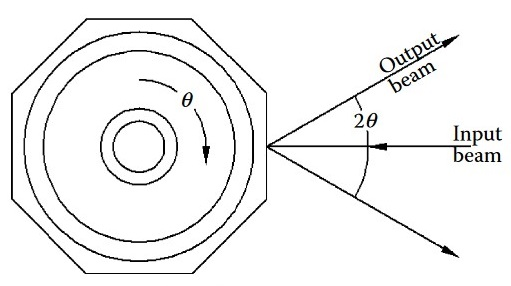
\includegraphics[width=0.5\textwidth]{img/polygon-scanner.jpg}
  \caption{\label{fig:polygon-scanner} mechanika polygonových skenerů}
\end{figure}

% \begin{figure}[!htb]
%   \centering
%   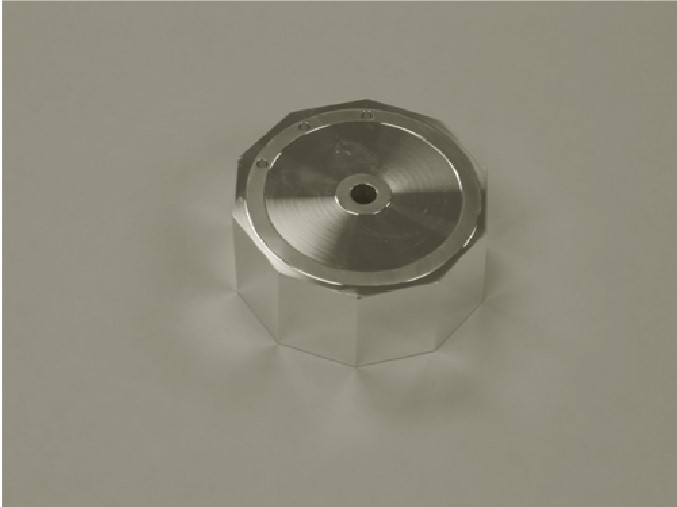
\includegraphics[width=0.5\textwidth]{img/polygon-prismatic-mirror.jpg}
%   \caption{\label{fig:polygon-prismatic-mirror} hranolové zrcátko polygonového skeneru}
% \end{figure}

% \begin{figure}[!htb]
%   \centering
%   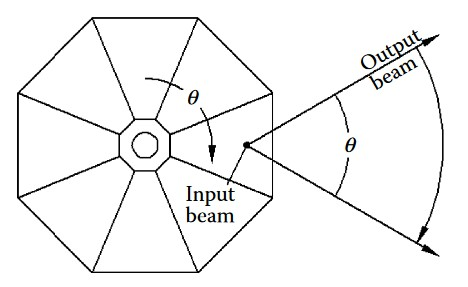
\includegraphics[width=0.5\textwidth]{img/polygon-pyramidal-mirror.jpg}
%   \caption{\label{fig:polygon-pyramidal-mirror} pyramidové zrcátko polygonového skeneru}
% \end{figure}
%

S jedním hranolem by hranolové skenery byly schopny směřovat paprsek pouze v jedné rovině - při projekci by bylo možné vykreslit maximálně čáru. Tuto limitaci lze kompenzovat přidáním melého rozdílu ve směřování každé strany hranolu, viz. obrázek \ref{fig:polygon-angular-variation}. S touto úpravou každá strana hranolu "vykreslí" jednu, svoji, přímku lehce posunutou vůči přímkách ostatních stran. Hranol s n-úhelníkovou podstavou je schopen vykreslit n přímek.
Další možností je kombinovat původní pravidelný hranol s galvanometrem (popsáno níže), kdy galvanometr nastaví jednu souřadnici paprsku a hranol na této souřadnici vykreslí přímku.

Tento typ skeneru se využívá hlavně pro senzory skenující na přímce (např. skenery čárových kódů~\cite{history-of-barcode-scanning}), nebo při rastrovém laser scanningu. Příklad rastrové projekce je vidět na obrázku \ref{fig:harddrive-projector-youtube}

\begin{figure}[!htb]
  \centering
  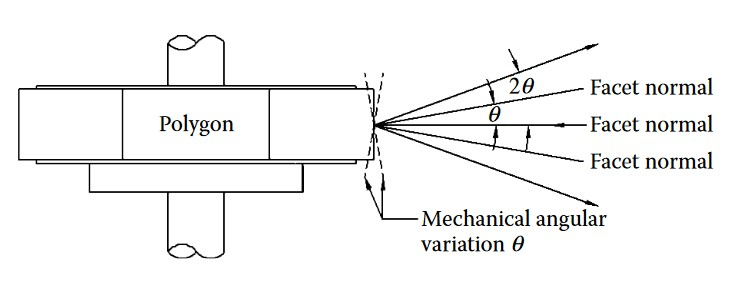
\includegraphics[width=0.8\textwidth]{img/polygon-angular-variation.jpg}
  \caption{\label{fig:polygon-angular-variation} úhlová rozdílnost polygonového skeneru}
\end{figure}


\begin{figure}[!htb]
  \centering
  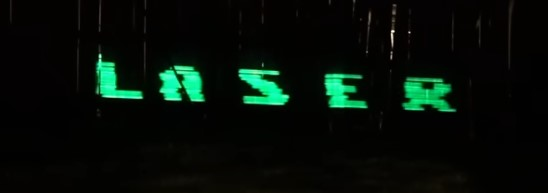
\includegraphics[width=0.5\textwidth]{img/harddrive-projection.jpg}
  \caption{\label{fig:harddrive-projection} příklad projekce laserového projektoru s polygonovým skenerem; zdroj \cite{harddrive-projector-youtube}}
\end{figure}

\section{Galvanometrové skenery}

Základní součástku galvanometrového skeneru je galvanometr.

\subsection{Galvanometr~\cite{some stuff}}      

\subsection{Konstrukce galvanometrových skenerů}
Jeden galvanometrový skener 

Narozdíl od hranolových skenerů je s galvanometrovým skenerem možné zastavit obě osy pohybu - vykreslovat na sebe kolmé čáry.

\begin{figure}[!htb]
  \centering
  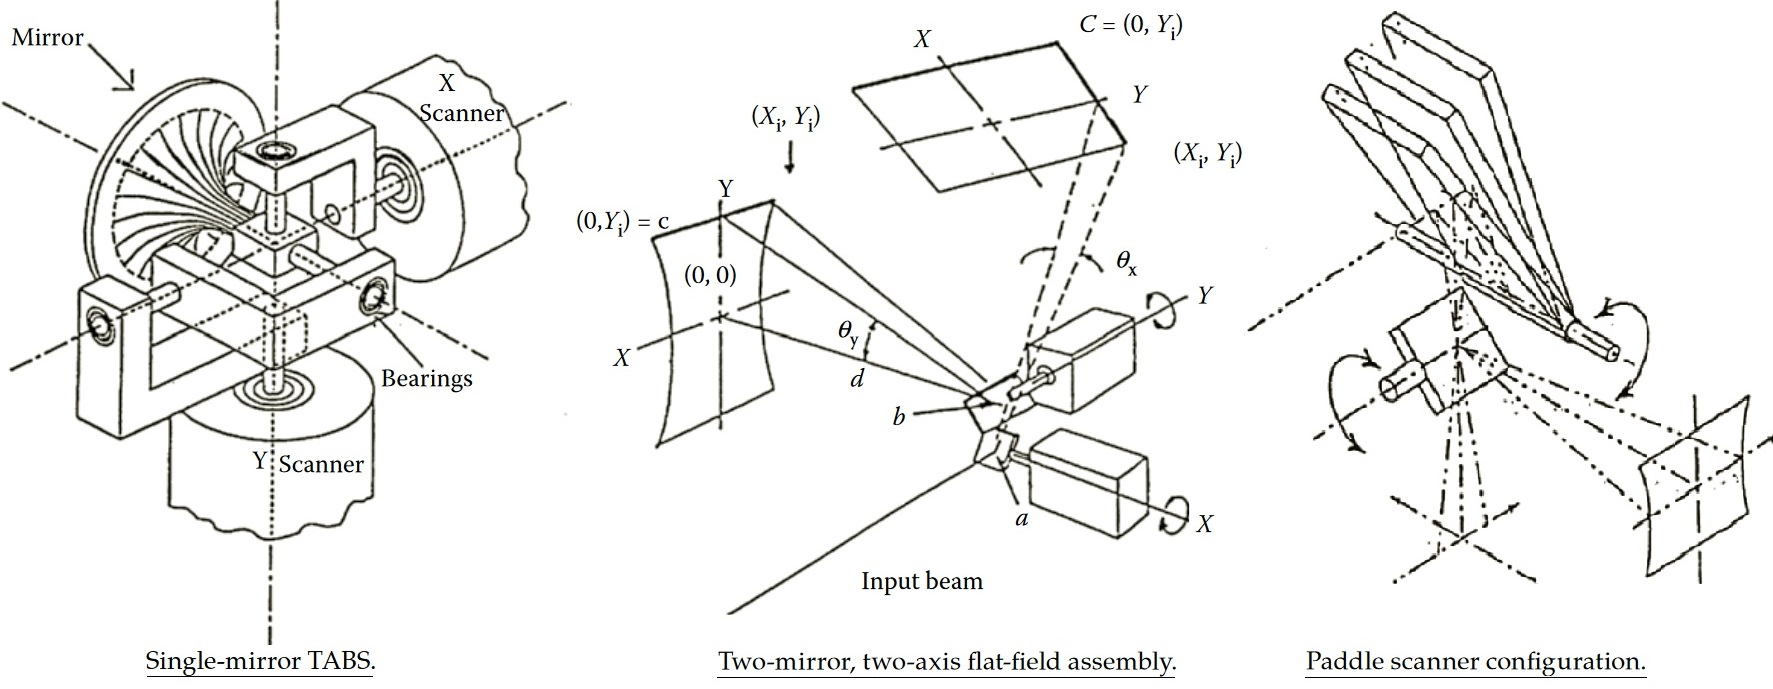
\includegraphics[width=1\textwidth]{img/scanner-constructions.jpg}
  \caption{\label{fig:scanner-constructions} různé konstrukce galvanometrových skenerů}
\end{figure}

\section{Má volba skeneru}

ja vyuzivam galva, protoze se s nima da nejlip pohrat, jsou nejuniverzalnejsi a tim padem nejvic zaujmou - cil

% \input{galvanometr.tex}

% \input{.tex}


\part*{praktická část}
\fxnote{wtf nechci, aby to  bylo vsechno na nove strance, kdo jsem?}
\addcontentsline{toc}{part}{praktická část} % přidá položku úvod do obsahu

\input{200-uvod-prak.tex}

% !TeX root = text.tex
\chapter{hardware}
Tato kapitola se zabývá fyzickou konstrukcí a zapojením vyrobeného laserového projektoru. Ten se skládá z řídící jednotky, galvanometrů s~ovládací elektronikou, laseru, chlazení a napájení. Všechny tyto součástky jsou uloženy v pouzdře vytisknutém na 3D tiskárně.

\section{Řídící jednotka -- Raspberry Pi}
\fxnote{TODO: rpi specs}

\section{Set galvanometrů se~zrcátky} \label{sec:my-galvos}
\subsection{Výběr skeneru}
Pro tuto práci byl vybrán galvanometrový skener, protože je~nejdostupnější a~protože potenciálním uživatelům nejlépe představí technologii.

Oproti hranolovým skenerům jim tožiž dává více možností, jak s paprskem pohybovat.
Můžou se~rozhodnout, že jej využijí jako hranolový skener, pokud nahrají soubor procházející promítací plochu po~řádcích.

Oproti dalším typům skenerů je~názornější, ostatní typy skenerů jsou totiž příliš malé a~není na~nich vidět princip funkce nebo je~jejich fungování nadmíru abstraktní a~těžko pochopitelné.

\subsection{Zapojení galvanometrového setu}
Samotné galvanometry jsou zapojeny do~řídící desky, která s nimi byla zakoupena, ta je vidět na obrázku~\ref{fig:hw_galvoboard}.

Řídící deska požaduje symetrický zdroj napětí 15~V, tzn. $+15$~V a~$-15$~V a~samozřejmě připojení k zemi. Také přijímá dva bipolární diferenciální analogové signály s~rozsahem diferenciálního napětí $-10$~V až $+10$~V. Každý signál udává vychýlení jednoho ze~dvou galvanometrů, což obvykle znamená výslednou pozici laserového paprsku v~osách X~a~Y.

\begin{figure}[htb]
  \centering
  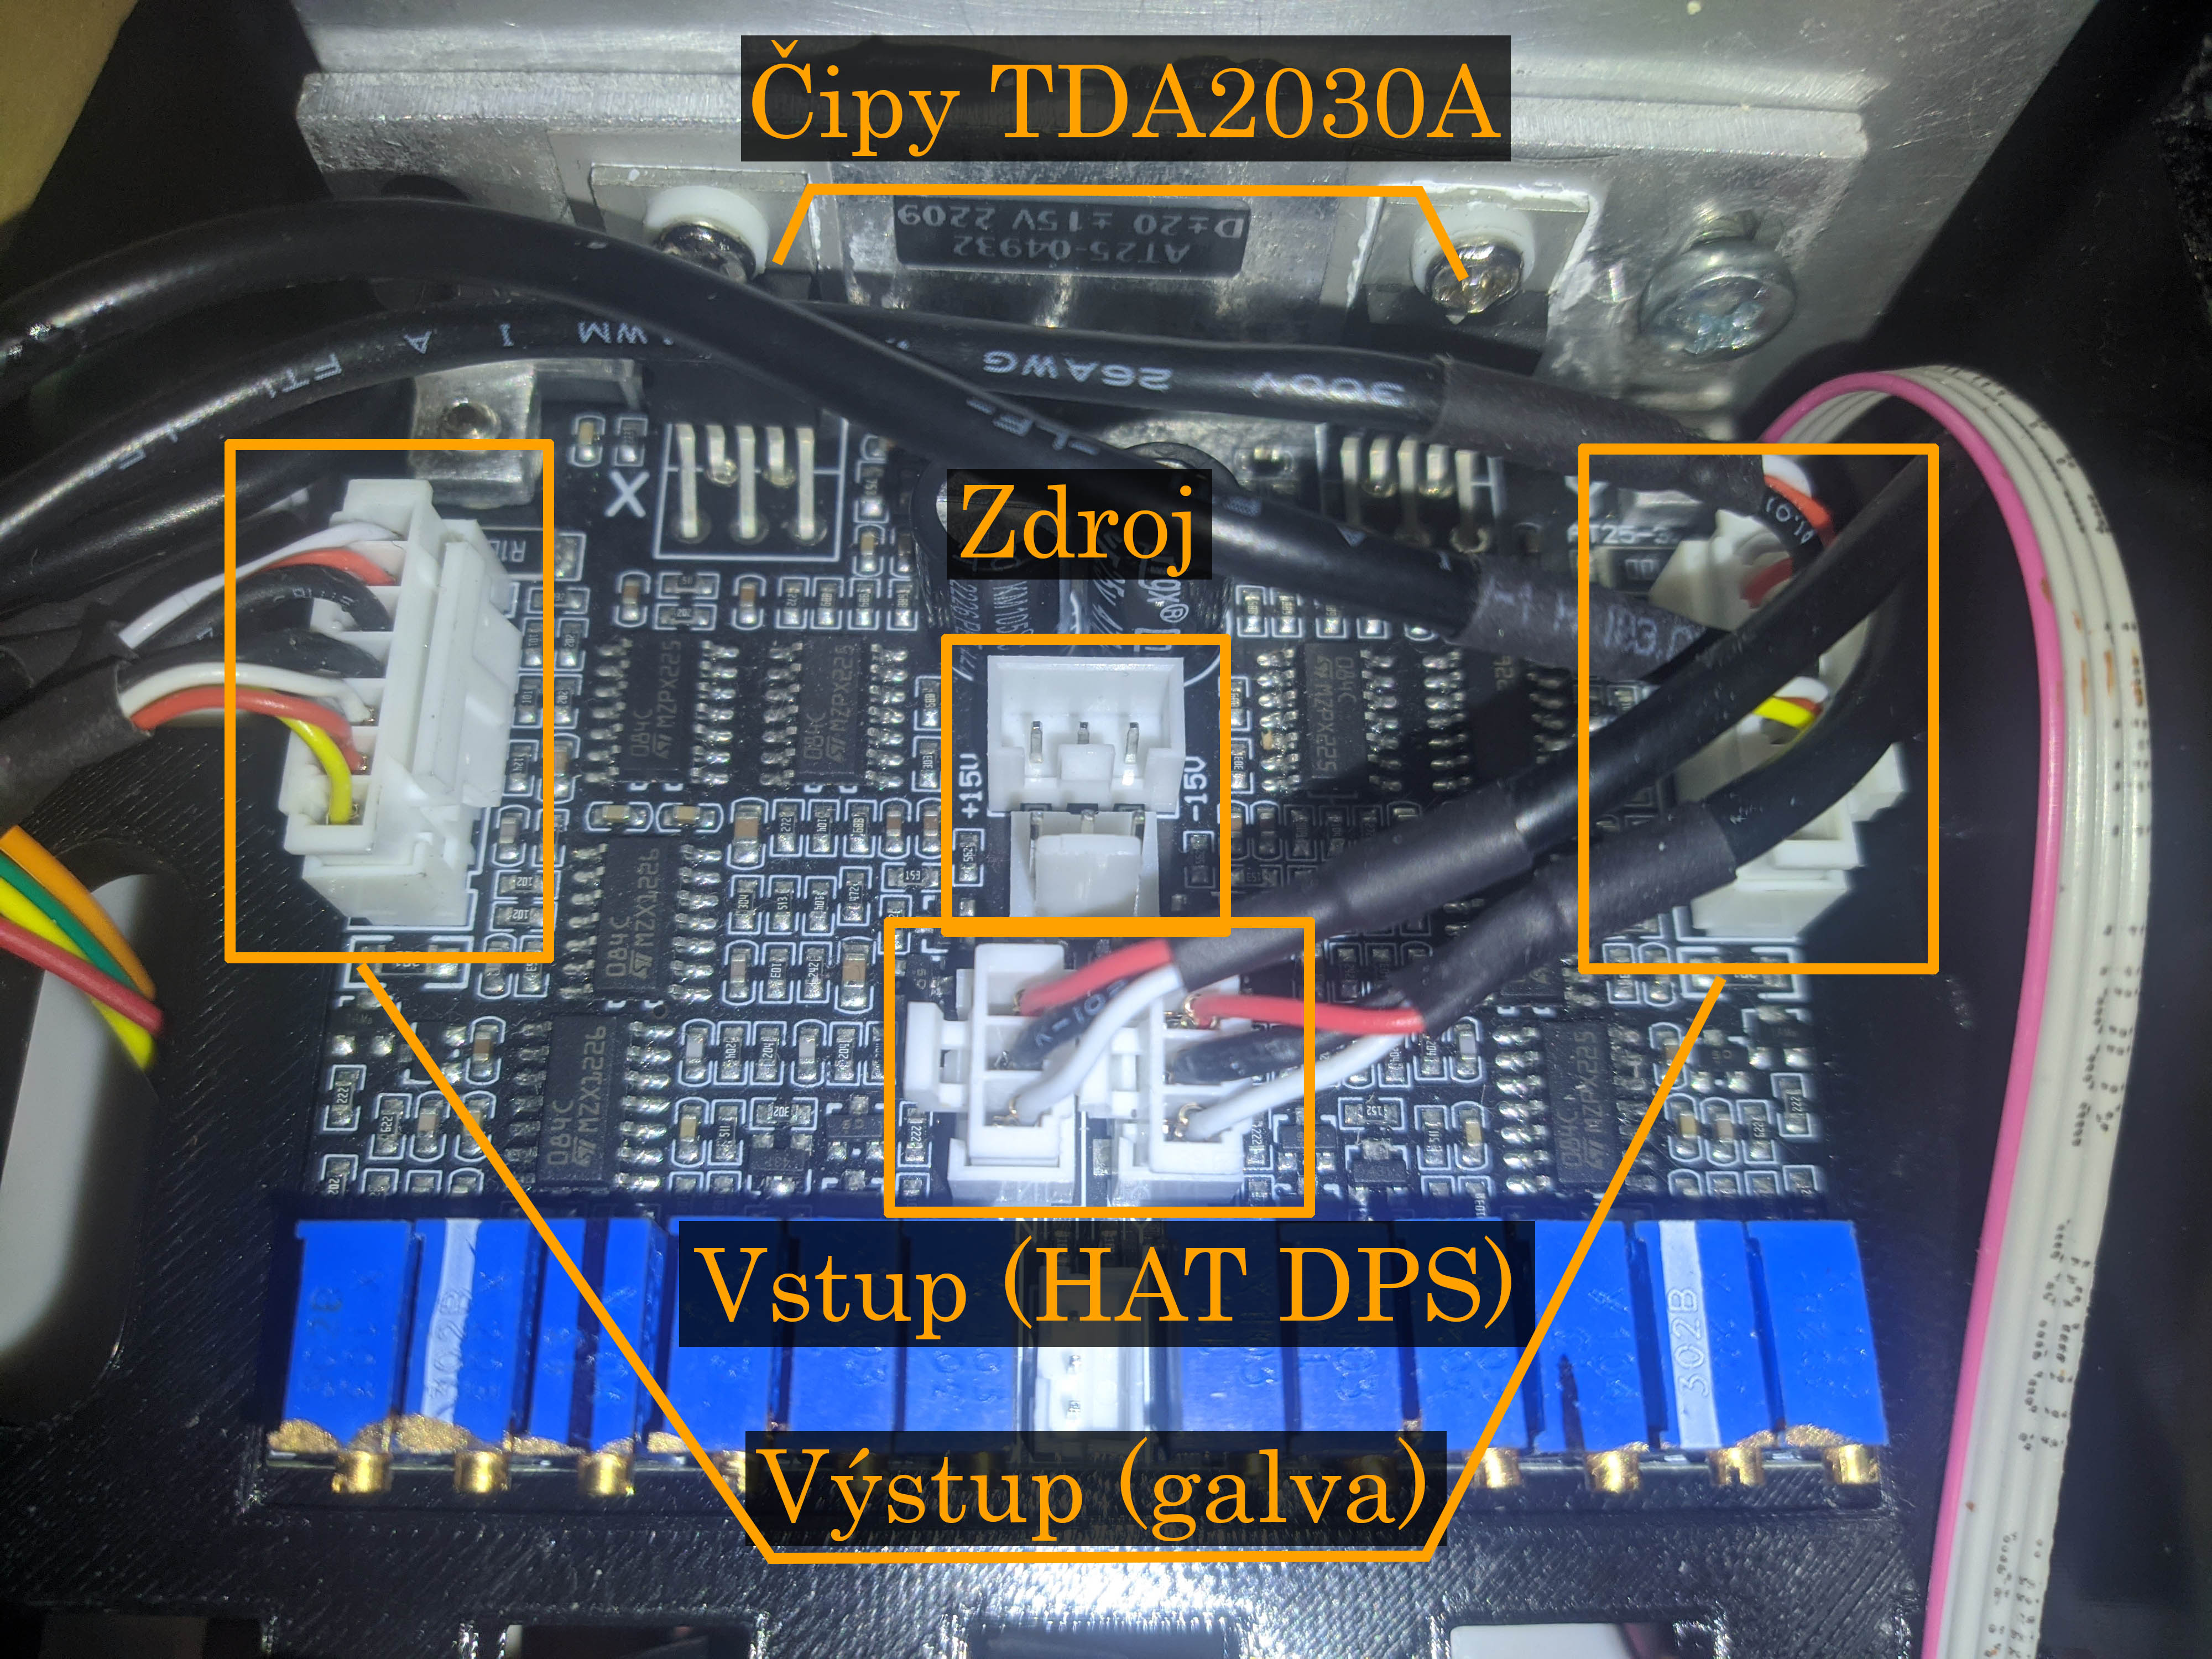
\includegraphics[width=1\textwidth]{img/hw_galvoboard.jpg}
  \caption{\label{fig:hw_galvoboard} Řídící deska galvanometrů s vyznačenými konektory a hřejícími čipy}
\end{figure}

\subsection{Bipolární diferenciální analogový signál}
Diferenciální signál je~signál přenášený dvěma vodiči, každý z~nich přenáší stejný signál, jen s~opačnou polaritou. Kontakt označený $(+)$ je~považován za~nosič základního signálu, zatímco kontakt označený $(-)$ je~považován za~nosič invertovaného signálu. Výsledné diferenciální napětí je~napětí na~základním nosiči vůči napětí na~obráceném nosiči, tzn.~$V_{dif} = V_{(+)} - V_{(-)}$.~\cite{ilda-signal-spec}

Bipolární signál znamená, že na~napětí každém z~kontaktů $(+)$ a~$(-)$ může dosahovat kladných i~záporných hodnot~\cite{ilda-signal-spec}.

Tudíž cheme-li disáhnout diferenciálního napětí $+10~V$, musí mít základní signál napětí $+5~V$ a~obrácený signál $-5~V$. Záporné diferenciální napětí bude ve~chvíli, kdy je~napětí základního signálu záporné a~napětí obráceného signálu kladné.

\subsection{Zahřívání čipů řídící desky galvanometrů} \label{sec:galvoboard-chips-heating-up}
Dva z~čipů na~řídící desce se při chodu systému výrazně zahřívájí. Na~tyto čipy je naštěstí už od~výroby desky připevněna malá hliníková destička. Ta~má sloužit jako chladič, ale i~s ní se~čipy v~otevřeném prostoru zahřívají na~teploty blízké 60~\degree{}C.
Dva zmíněné čipy jsou čipy TDA2030A od~firmy STMicroelectronics. Ty~by~měly dle datasheetu vydržet až 150~\degree{}C, ale dá se~předpokládat, že v~uzavřeném pouzdru budou čipy dosahovat vyšších teplot, než v~otevřeném prostoru. I~kdyby nedosáhly pro sebe kritických 150~\degree{}C, rozhodně není žádoucí, aby uvnitř projektoru desky dosahovaly vysokých teplot.

I proto byl do~projektoru zabudován chladič. Více o~způsobu jeho připevnění a~distribuci chlazení mezi ostatní komponenty se~dočtete v~kapitole~\ref{sec:krabick-design-priorities}.


\section{laser}
Jako zdroj laserového paprsku byl využit RGB laserový modul, skládající se ze tří barevných diod a dichroických zrcátek.

\subsection{Dichroická zrcadla~\cite{dichronic-mirrors}}

\fxnote{TODO: slouzi k}

Dichroická zrcadla jsou zrcadla s výrazně rodílnými odrazovými nebo průchodovými vlastnostmi pro dvě různé vlnové délky odraženého~/~procházejícího světla.

Většina dichroických zrcadel jsou dielektrická zrcádla \footnote{Dielektrická zrcadla jsou zrcadla, skládající se z mnoha tenkých vrstev různě opticky propustných materiálů.}, existují ale také krystalická zrcadla\footnote{Krystalická zrcadla jsou zrcadla, jejiž odrážlivá vrstva se skládá z monokrystalického materiálu, typicky polovodiče.}.


\section{Displej z~tekutých krystalů (LCD)}
Pro zobrazování informací uživateli přímo na~zařízení byl~využit alfanumerický\footnote{Alfanumerický -- Řídící jednotka displeji místo pixelů posílá celé znaky, které sám vykresluje.} LCD~s řadičem HD44780 a~s~rozlišením 20~x~4 znaky. K~displeji je~také připojen I$^{2}$C převodník, který slouží jako prostředník mezi řadičem displeje a~Raspberry Pi.
Komunikační protokol LCD~totiž využívá podstatně více kontaktů, než I$^{2}$C sběrnice, kterou Raspberry Pi~komunikuje s~převodníkem.
% Převodník je~k~pinům Raspberry Pi~připojen dle~tabulky~\ref{tab:LCD_conn}.

\begin{figure}[htb]
  \centering
  \begin{minipage}{0.45\textwidth}
    \centering
    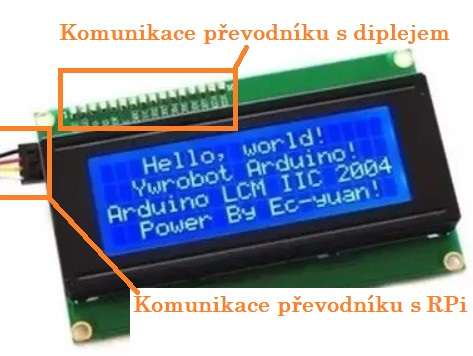
\includegraphics[width=1\textwidth]{img/LCD_front.jpg} % first figure itself
    \caption{\label{fig:LCD_front} Displej z~tekutých krystalů (LCD); Převzato a~upraveno z~\cite{laskakit-LCD}}
  \end{minipage}\hfill
  \begin{minipage}{0.45\textwidth}
    \centering
    \includegraphics[width=1\textwidth]{img/LCD_back.jpg} % second figure itself
    \caption{\label{fig:LCD_back} I$^{2}$C převodník napojený na~LCD~\cite{laskakit-LCD}}
  \end{minipage}
\end{figure}

% \begin{table}[htb]
%   \centering
%   \begin{tabular}{c|c}
%     kontakt převodníku & kontakt RPi~\\
%     \hline
%      GND~               & GND~        \\
%     5V                 & 5V          \\
%      SCK~               & GPIO3       \\
%      SDA~               & GPIO2       \\
%      LED~               & GPIO18      \\
%   \end{tabular}
%   \caption{\label{tab:LCD_conn} Připojení kontaktů I$^{2}$C převodníku na~kontakty RPi.}
% \end{table}


\section{Rotační enkodér}
Rotační enkodér je~typ~pozičního senzoru používaný k~měření rotace otáčivé hřídele~\cite{how-encoders-work}. Existuje mnoho druhů enkodérů, rozdělují se~dle~signálu, který vydávají a~dle~technologie, kterou měří rotaci hřídele~\cite{how-encoders-work}. V~této práci je~použit mechanický inkrementální enkodér s~tlačítkem.

Na obrázku~\ref{fig:encoder-working} je~vidět, jak~enkodér funguje uvnitř. Dva~kontakty A~a~B při rotaci získávají a~ztrácí kontakt s~kontaktem C. Připojíme-li ke~kontaktu C~zem a~ke~kontaktům A~a~B pull-up rezistory (klidně softwarově), dá se~toto získávání a~ztrácení kontaktu zaznamenat do~grafu na~obrázku~\ref{fig:encoder-graph} jako dva~signály obdélníkového průběhu vzájemně fázově posunuté o~90 stupňů.

\begin{figure}[htb]
  \centering
  \begin{minipage}{0.45\textwidth}
    \centering
    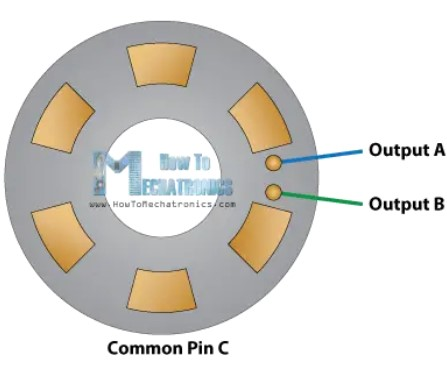
\includegraphics[width=1\textwidth]{img/encoder-working.jpg}
    \caption{\label{fig:encoder-working} Vnitřní schéma enkodéru~\cite{how-encoders-work}}
  \end{minipage}\hfill
  \begin{minipage}{0.45\textwidth}
    \centering
    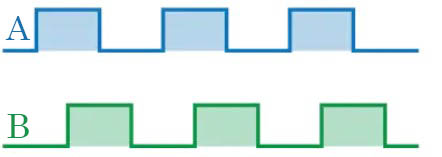
\includegraphics[width=1\textwidth]{img/encoder-graph.jpg}
    \caption{\label{fig:encoder-graph} Výstup enkodéru~\cite{how-encoders-work}}
  \end{minipage}
\end{figure}

Použitý rotační enkodér má další dva~kontakty připojené k~tlačítku pod~rotující hřídelí.
Ke~čtení stisknutí tlačítka je~potřeba připojit jeden kontakt k~zemi, tedy ke~kontaktu C~a~druhý kontakt na~pull-up rezistor (klidně softwarově).
Celé zapojení enkodéru je~naznačeno na~obrázku~\ref{fig:encoder-pinout}. Kontakty tlačítka jsou v~něm označeny S1 a~S2.
% Enkodér je~k~RPi připojen dle~tabulky~\ref{tab:enc_conn}.

% \begin{table}[htb]
%   \centering
%   \begin{tabular}{c | c}
%     kontakt enkodéru & kontakt RPi~\\
%     \hline
%      C~               & GND~        \\
%     S2               & GND~        \\
%     A~               & GPIO5       \\
%      SDA~             & GPIO6       \\
%     S1               & GPIO13      \\
%   \end{tabular}
%   \caption{\label{tab:enc_conn} Připojení kontaktů rotačního enkodéru na~kontakty RPi.}
% \end{table}


\subsection{Čtení pozice z~rotačního enkodéru}
U rotačního enkodéru se~při každé otáčce změní připojení pinů několikkrát. Chceme-li pozorovat pouze počet těchto změn, stačí spočítat změny na~jednom kontaktu. Pokud je~ale~zapotřebí pozorovat i~směr otáčení, je~nutné pozorovat stav obou kontaktů. Pokud se~enkodér otáčí po~směru hodinových ručiček, kontakt A~bude fázově posunut o~90 stupňů napřed oproti kontaktu B.
Pokud se~eknodér otáčí proti směru hodinových ručiček, bude naopak kontakt B~o 90 stupňů napřed oproti kontaktu A. Časový průběh stavu kontaktů je~naznačen na~obrázku~\ref{fig:encoder_data}.
\begin{figure}[htb]
  \centering
  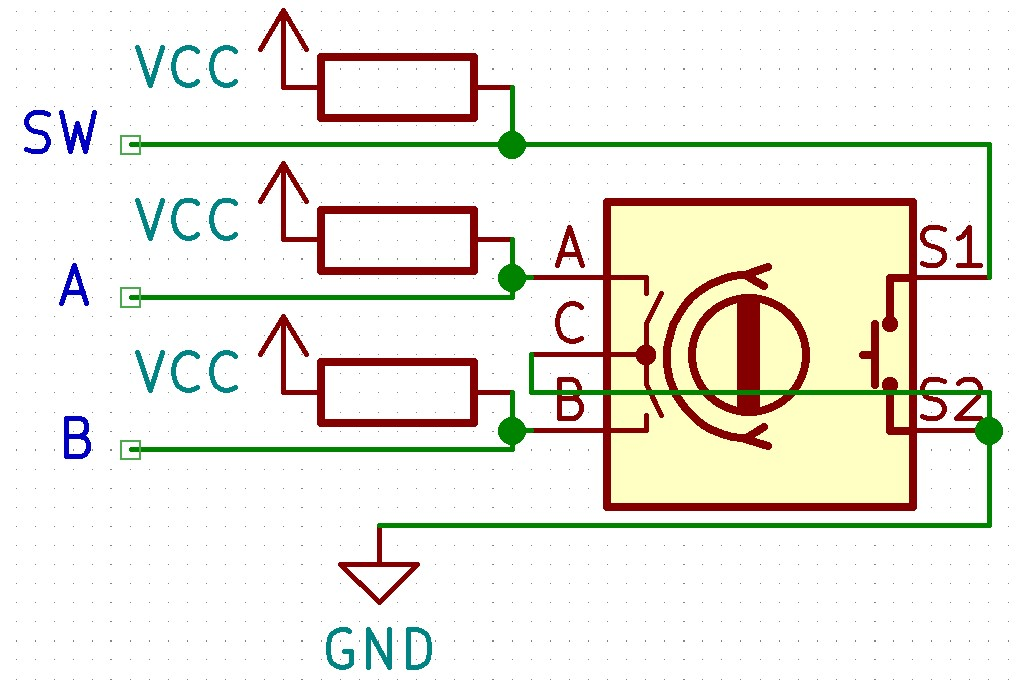
\includegraphics[width=0.5\textwidth]{img/encoder-pinout.jpg}
  \caption{\label{fig:encoder-pinout} Schéma zapojení rotačního enkodéru.}
\end{figure}
\begin{figure}[htb]
  \centering
  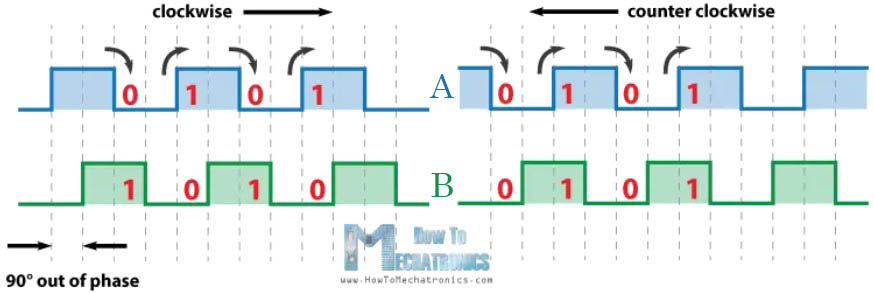
\includegraphics[width=1\textwidth]{img/encoder_data.jpg}
  \centering
  \caption{\label{fig:encoder_data} Časový průběh stavu kontaktů rotačního enkodéru při otáčení hřídelí na~obě strany}
\end{figure}


\section{HAT deska plošných spojů}
Pro ovládání výše popsaného hardwaru je~zapotřebí několik specifických obvodů.
Kvůli jejich specifičnosti tyto obvody nejsou volně dostupné k~zakoupení na~předem vytvořených destičkách. Proto bylo zapotřebí je~z~jednotlivých součástek vyrobit na~míru.

Obvody byly navrženy v~programu KiCad, celé schéma desky je k nalezení mezi přílohami s označením~\ref{fig:pcb-schematic-full}. Následně pro ně v~tomtéž programu byla nadesignována deska plošných spojů. Mezi obvody patří:
\begin{itemize}
  \item Zdroj $-15$~V pro galvanometry.
  \item Generátor signálu pro řídící desku galvanometrů.
  \item Voltmetr baterií.
\end{itemize}

Kromě nich byly na~desku přidány konektory k~jednotlivým barevným vstupům laseru, LCD displeji a~k rotačnímu enkodéru, které jsou přímo napojeny na~40 pinový GPIO konektor Raspberry Pi.
Deska byla designována jako tzv. HAT, to~znamená, že sama na~tomto konektoru drží a~nezabírá o~moc víc místa, než samotné Raspberry Pi.
\fxnote{TODO: obrazek desky (maybe mounted) (deska ještě nedošla)}

\subsection{Zdroj $-15$~V}\label{sec:negative-ps}
Napětí $-15$~V je získáváno obvodem napěťového invertoru založeném na obvodu ze zdroje~\cite{ampalyzer}. Jeho zapojení je na obrázku~\ref{fig:negative-ps}, potřebuje zdroj napětí 15V.

\begin{figure}[htb]
  \centering
  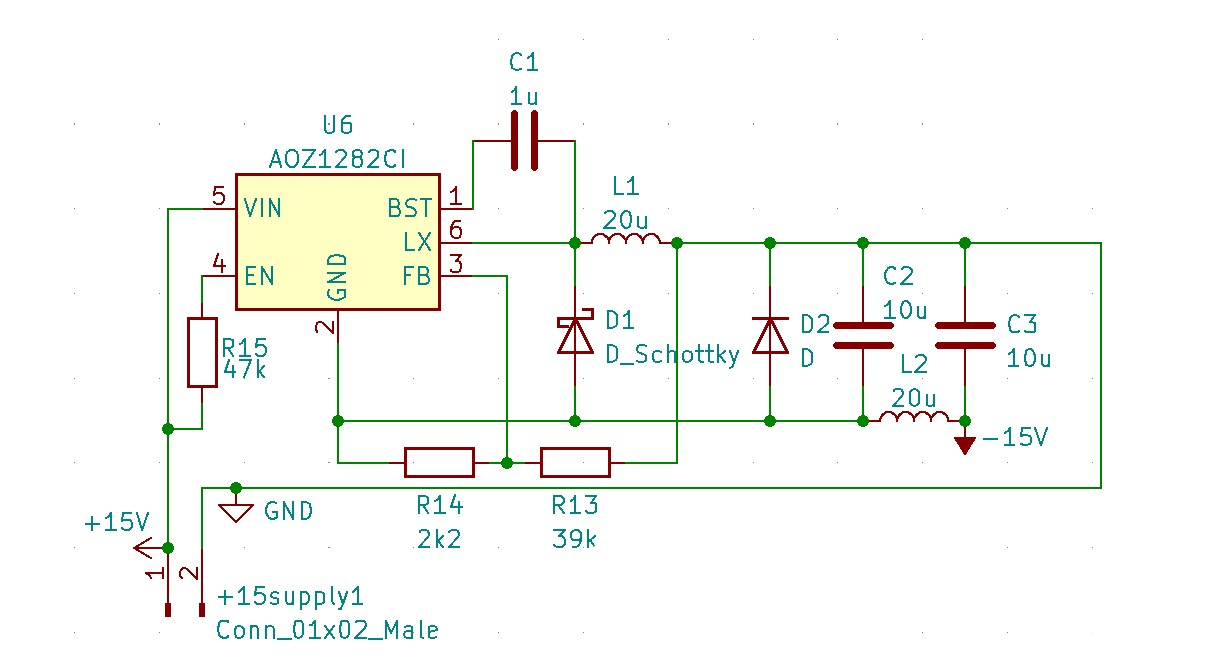
\includegraphics[width=0.9\textwidth]{img/negative-ps.jpg}
  \caption{\label{fig:negative-ps} Zapojení invertujícího obvodu}
\end{figure}

Centrem obvodu je integrovaný obvod AOZ1282 od výrobce Alpha \& Omega Semiconductor označený U6. Tento integrovaný obvod obsahuje spínací transistor (ve zjednodušeném schématu prvek SW), PWM regulační obvod pracující na frekvenci 450 kHz s napěťovou referencí 0,8 V, který reguluje čas připojení induktoru L1.
K němu je připojen bootstrapový kondenzátor C1, ten zajišťuje plovoucí buzení pro integrovaný spínač.
Dále je k němu připojený výkonový induktor L1, jehož hodnota byla zvolena dle rovnic uvedených ve zdroji~\cite{basic-calc-boost}, respektive podle dále uvedené rovnice~\ref{equ:inductor-calc}.~\cite{ampalyzer}

\begin{equ}[H]
  \centering
  \begin{math}
    L = \frac{-U_{OUT}\times U_{IN}}{0,4 \times 2 \times I_{OUT} \times f_{s} \times \left ( U_{IN} - U_{OUT} \right )} = \frac{- \left (-15 V \right )\times 15 V}{0,4 \times 2 \times 1 A \times 450 kHz \times \left ( 15 V - \left (-15 V \right ) \right )} \approx 21 \mu H
  \end{math}
  \caption{\label{equ:inductor-calc} Výpočet ideální indukčnosti cívky pro invertující obvod}
\end{equ}

\It{
  L --- Indukčnost spínaného induktoru \\
  U$_{IN}$ --- Vstupní napětí do invertujícího obvodu \\
  U$_{OUT}$ --- Výstupní napětí z invertujícího obvodu \\
  I$_{OUT}$ --- Výstupní proud z invertujícího obvodu \\
  f$_{s}$ --- Frekvence spínacího regulátoru \\
}

Na FB pin integrovaného obvodu je připojen napěťový dělič tvořený odpory R13 a R14, který integrovanému obvodu dodává zpětnou vazbu o výstupním napětí.
Hodnoty R13 a R14 jsou voleny tak, aby při 15 V, tedy požadovaném výstupním napětí, bylo na výstupu děliče napětí 0,8 V, tedy referenční napětí integrovaného spínaného regulátoru.
Schottkyho dioda SS56, označená D1, slouží k zadržení změny polarity induktoru. Usměrňovací dioda D2 je v propustném stavu při prvotním spuštění měniče, kdy je přes ní napájen U1 po dobu náběhu výstupního záporného napětí.
Posledním prvkem je výstupní vyhlazovací filtr tvořený kondenzátory C3 a C4 společně s induktorem L2.
Jeho úkol je minimalizovat výstupní napěťového zvlnění zdroje.~\cite{ampalyzer}

\subsection{Generátor analogového signálu}\label{sec:ilda-signal-gen}
Jak je popsáno v~sekci~\ref{sec:my-galvos}, řídící deska galvanometrů přijmá dva bipolární diferenciální analogové signály v~rozpětí $-5$~V až $+5$~V.

Obvod, který se~stará o~vytváření tohoto signálu, je~založený na~obvodu ze~zdroje~\cite{lasershow-with-real-galvos}.
Vytváření tohoto signálu je~rozděleno do~dvou částí. Nejdříve D/A~převodník připojený k~RPi vytvoří signál v~rozpětí 0 až 5~V a~následně je~tento signál pomocí invertujících operačních zesilovačů převeden na~požadované rozpětí a invertován.
Jednotlivé části tohoto obvodu jsou blíže popsány v~následujících kapitolách.

\subsubsection{D/A převodník}
K generování signálu v~rozpětí 0--5~V byl využit dvoukanálový D/A převodník\footnote{D/A převodník je obvod, který na~základě instrukcí přijatých digitálně generuje analogové napětí.} MCP4822.
Tento čip podporuje komunikaci přes rozhraní SPI, pracuje s~napájecím napětím 5~V a~s 12bitovým rozlišením (je schopen vygenerovat 4~096 různých napětí) na~dvou kanálech~\cite{mcp4822-dsh}.
RPi komunikuje s~čipem pomocí rozhraní SPI popsaném v kapitole~\ref{sec:spi}.

\subsubsection{Operační zesilovače~\cite{tl082-dsh}}
K modifikaci signálu z~DAC na~bipolární diferenciální analogový signál slouží pro každý kanál jeden čip TL082, který obsahuje dva operační zesilovače. Ty~jsou zapojeny dle schématu na~obrázku~\ref{fig:ilda_amps-scheme}.

Signál první operační zesilovač zesílí/zeslabí a~vertikálně posune dle nastavení potenciometrů Ygain (zesílení) a~Yoffset (posun) a~zároveň invertuje. Tento invertovaný signál následně druhý operační zesilovač opět invertuje. Tím získavá základní signál pro řídící desku galvanometrů.

\begin{figure}[htb]
  \centering
  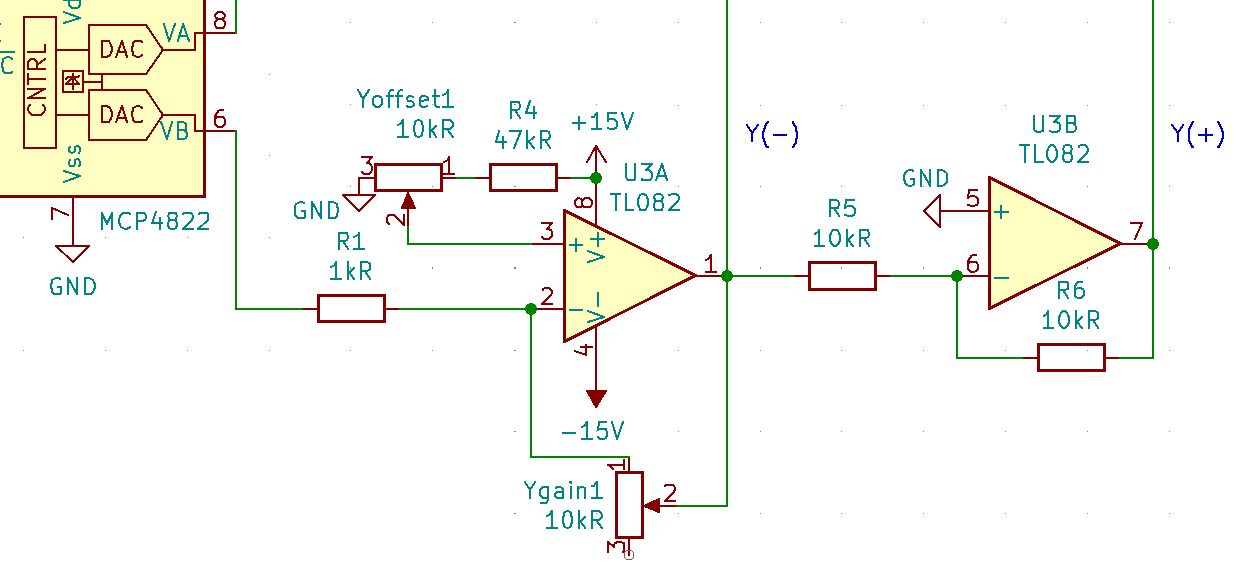
\includegraphics[width=1\textwidth]{img/ilda_amps.png}
  \caption{\label{fig:ilda_amps-scheme} Zapojení čipu TL082 pro jeden kanál řídící desky galvanometrů}
\end{figure}

\subsection{Voltmetr baterií}
Obvod voltmetru baterií je vidět na obrázku \ref{fig:bat_probe}.

\begin{figure}[htb]
  \centering
  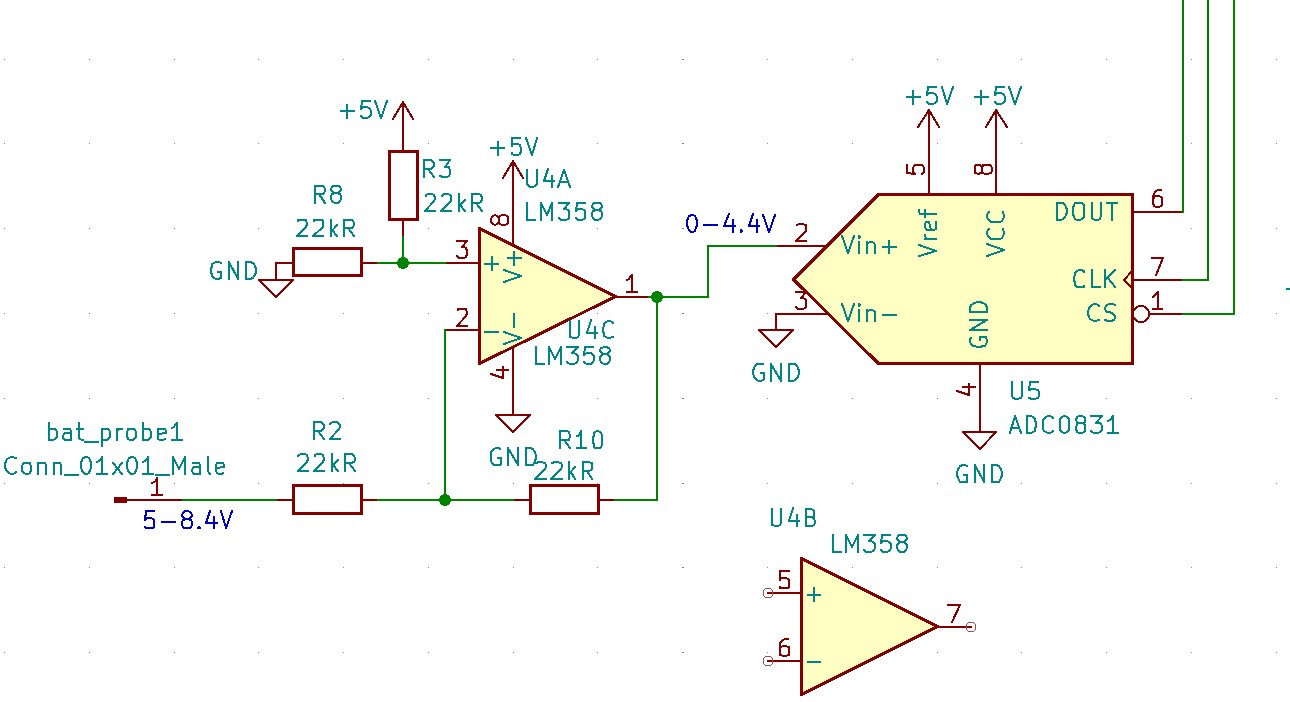
\includegraphics[width=0.6\textwidth]{img/bat_probe.jpg}
  \caption{\label{fig:bat_probe} Schéma obvodu voltmetru baterie}
\end{figure}

Jako voltmetr baterií slouží A/D převodník ADC0831 od firmy Texas Instruments Incorporated~\cite{adc0831-dsh}. Ten je označen U5 a je zapojen společně s operačním zesilovačem LM358 od stejného výrobce, který je označen U4.
Operační zesilovač je zapojen jako rozdílový zesilovač podle zdroje~\cite{odcitacka} tak, aby od napětí baterií, které se může pohybovat v rozsahu 6~V až 8,4~V, odečítal 5~V.
Díky tomu se napětí, která měří A/D převodník pohybují mezi hodnotami 1~V a 3,4~V. S jeho osmibitovým rozlišením a referenčním napětím 5~V v tomto rozpětí může naměřit 122 různých napětí.

A/D převodník tyto data posílá do Raspberry Pi pomocí rozhraní SPI a to s nimi dále pracuje.


\section{Napájení}
Celkové schéma napájení je vidět na obrázku~\ref{fig:power-schem-full}.

\begin{figure}[!h]
  \centering
  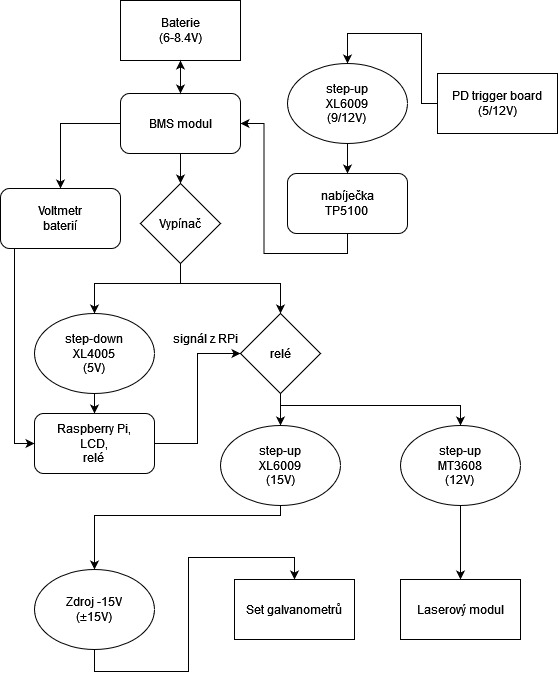
\includegraphics[width=\textwidth]{img/power-schem-full.jpg}
  \caption{\label{fig:power-schem-full} Celkové schéma napájení komponentů projektoru}
\end{figure}

\subsection{Akumulátory}
K napájení projektoru byly využity 4 Lithium-iontové akumulátory Samsung INR 18650 s kapacitou 3450~mAh a jmenovitým napětím 3.7~V. Ty byly zapojeny nejdříve po dvojicích paralelně a následně byly tyto dvojice zapojeny sériově. Konečný článek tedy dosahuje jmenovitého napětí 7,4~V.

\subsection{BMS modul}
Na baterie byl napojen ochranný BMS (Battery management system) modul, který ji chrání před následujícími stavy:
\begin{itemize}
  \item odběr vysokého proudu (zkrat)
  \item přebití
  \item vybití
  \item nevybalancované články
\end{itemize}
Modul články balancuje a v případě, že nastane jiný z nežádoucích stavů, ji odpojí. Modul je na obrázku \ref{fig:BMS}


\begin{figure}[htb]
  \centering
  \begin{minipage}{0.45\textwidth}
    \centering
  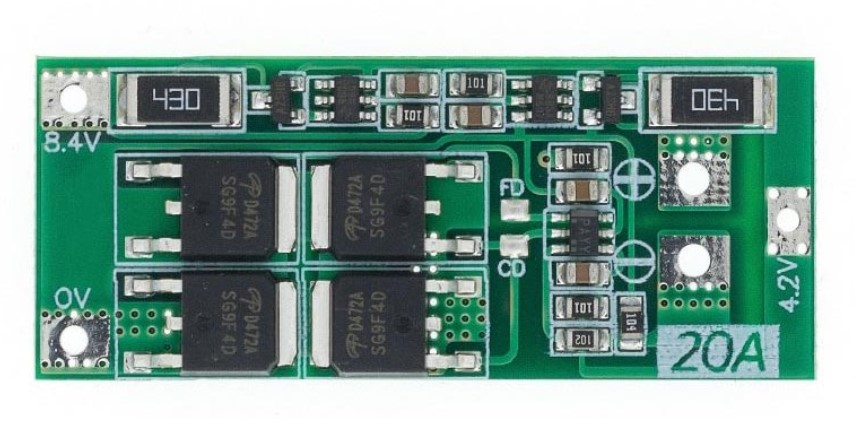
\includegraphics[width=0.8\textwidth]{img/BMS.jpg}
  \caption{\label{fig:BMS} BMS Modul se třemi kontakty pro sérii baterií (0V, 4.2V a 8.4V) a výstupními kontakty ($(+)$ a $(-)$); Převzato z~\cite{laskakit-BMS}}
  \end{minipage}\hfill
  \begin{minipage}{0.45\textwidth}
    \centering
  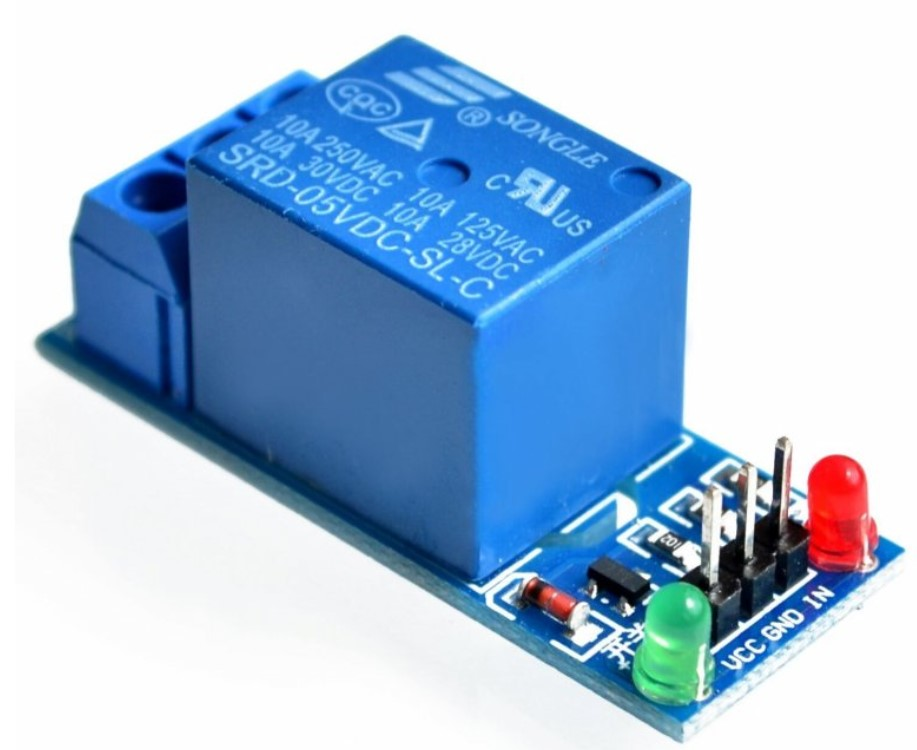
\includegraphics[width=0.8\textwidth]{img/relay.jpg}
  \caption{\label{fig:relay} Relé modul; Převzato z~\cite{laskakit-relay}}
  \end{minipage}
\end{figure}

\subsection{relé modul}
V projektoru byl využit relé modul pro připojování komponentů s vysokým odběrem pouze ve chvílích, kdy jsou využívány. Jedná se o set galvanometrů, laserový modul a větrák, ty jsou připojeny jen ve chvílích, kdy projektor promítá.

Relé modul je ovládán jedním kontaktem spojeným s Raspberry Pi a je umístěn mezi bateriemi a měniči napětí, proto stačí pouze jeden na více napěťových větví. Je vidět na obrazku~\ref{fig:relay}

\subsection{nabíjecí obvod}
Zapojený nabíjecí obvod je vidět na obrázku~\ref{fig:hw_charging_circuit}.

\begin{figure}[htb]
  \centering
  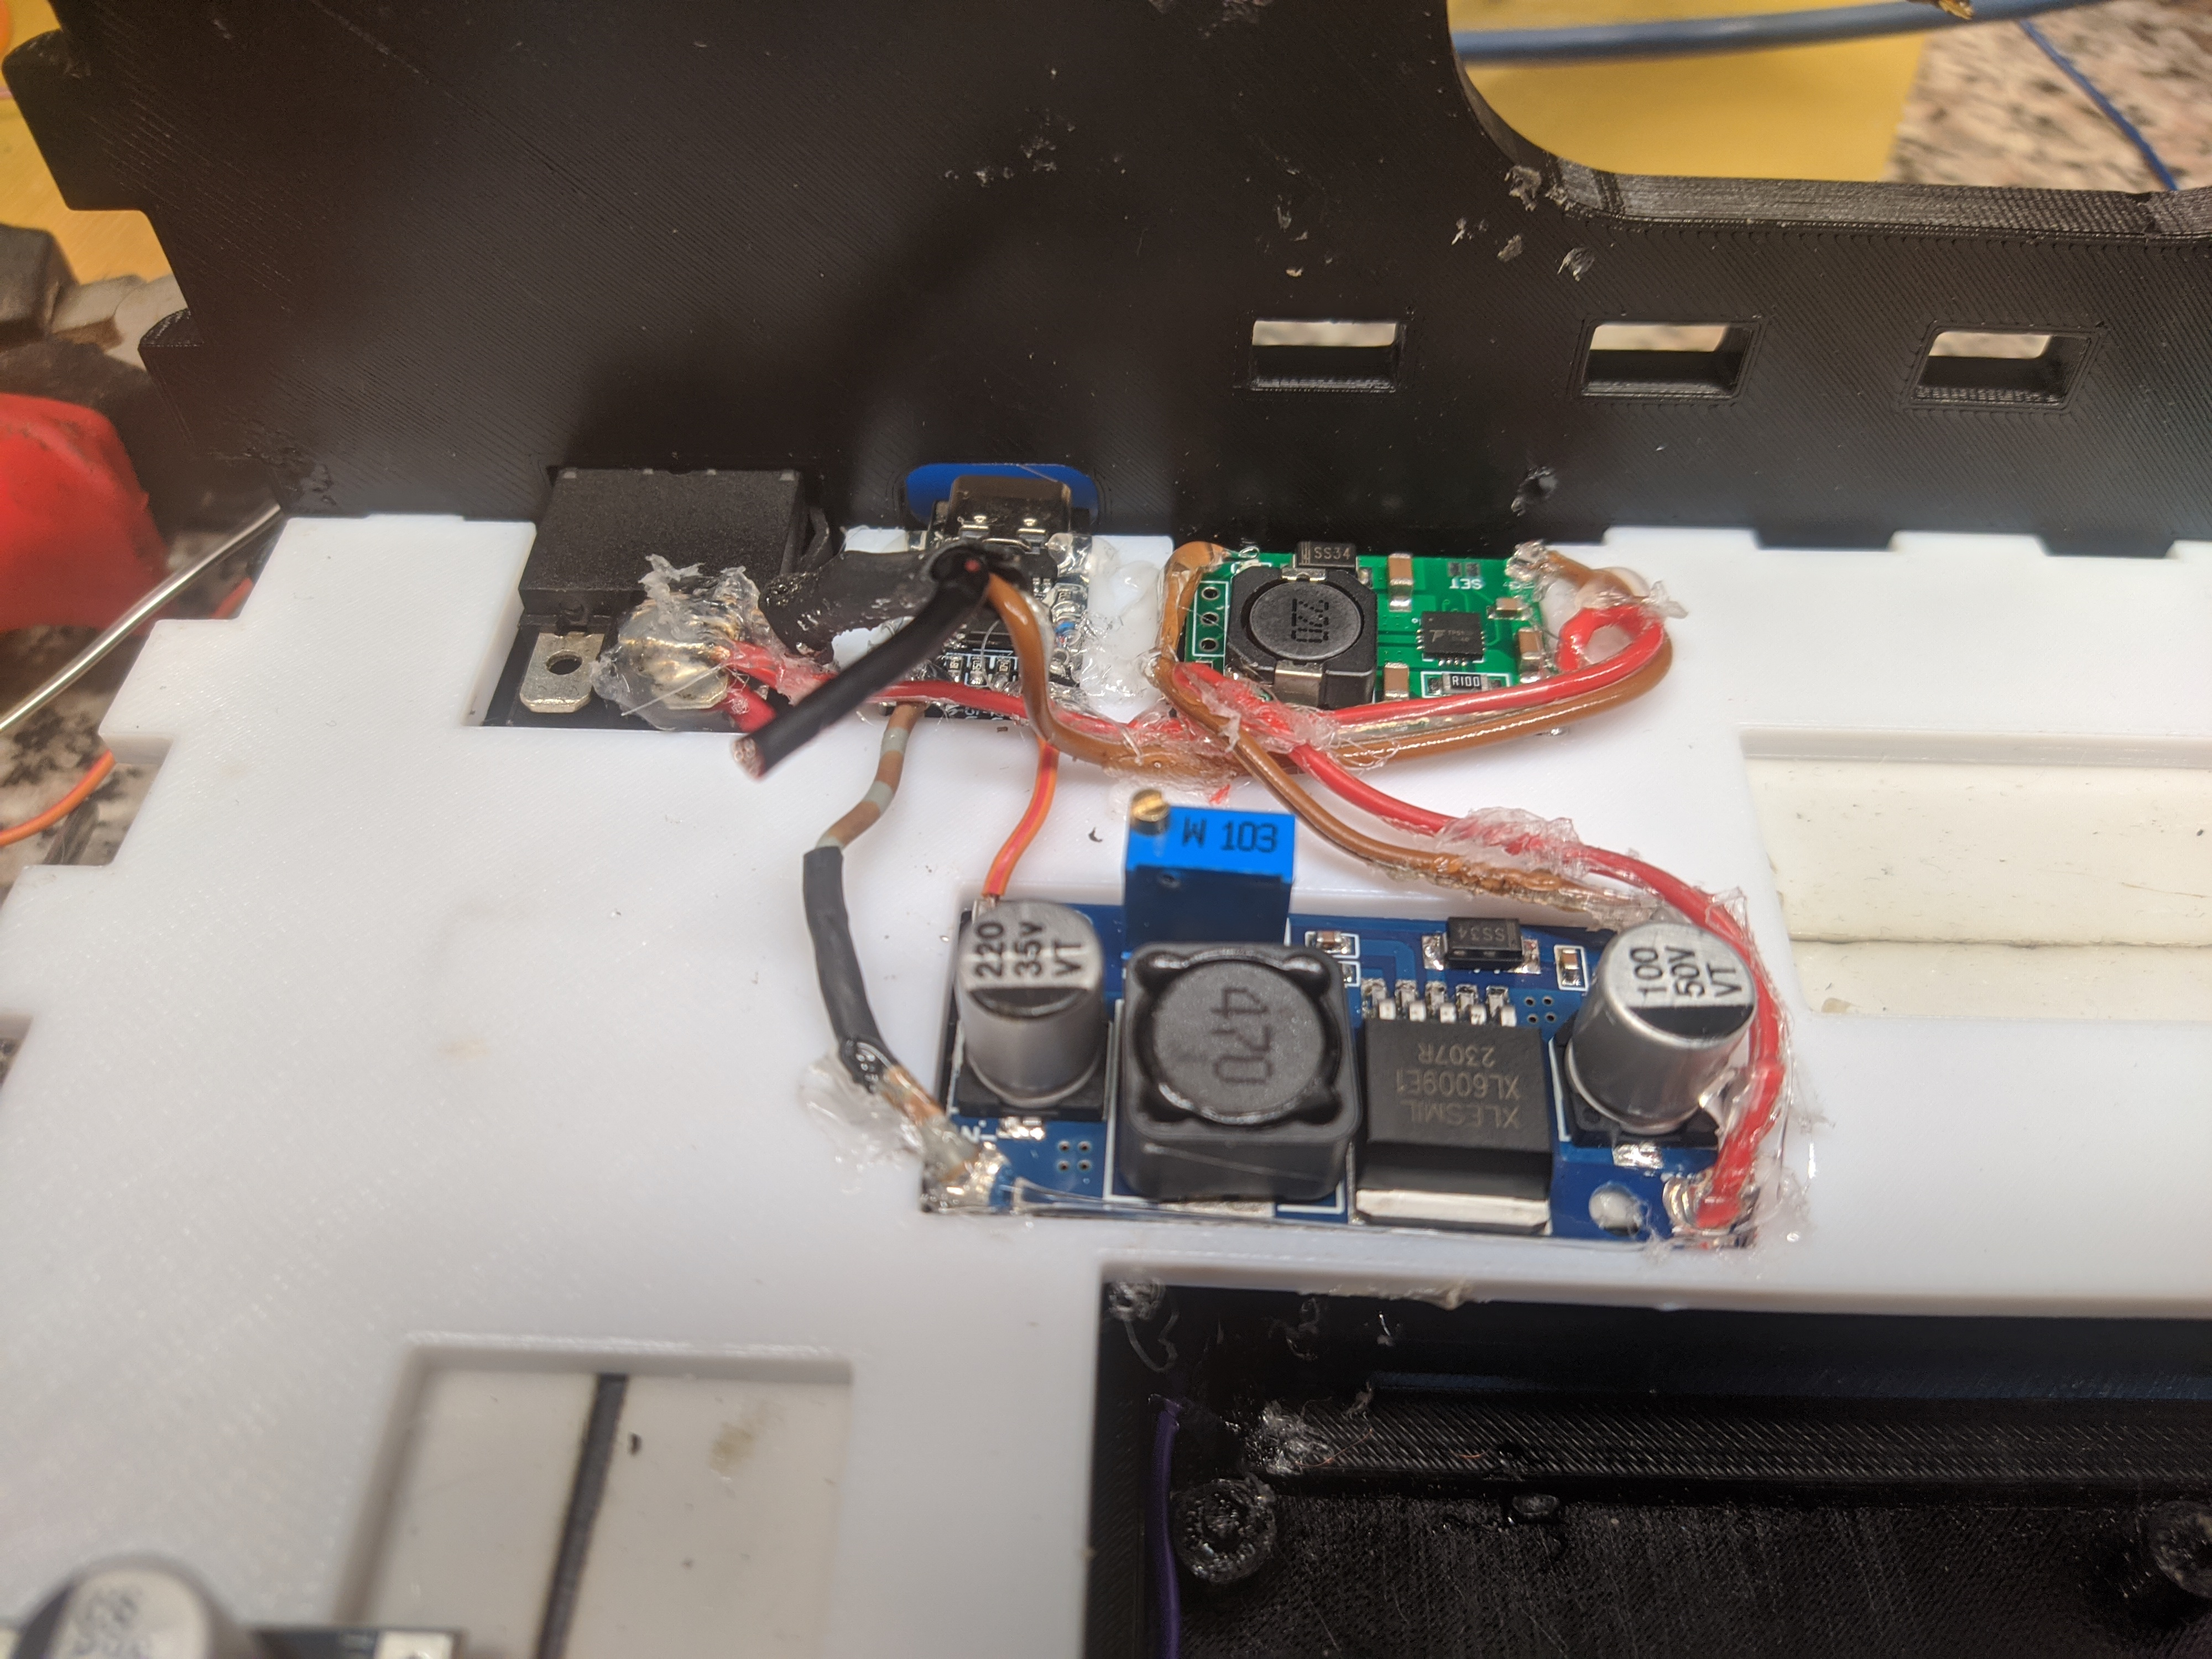
\includegraphics[width=0.8\textwidth]{img/hw_charging_circuit.jpg}
  \caption{\label{fig:hw_charging_circuit} Zapojený nabíjecí obvod}
\end{figure}

\subsubsection{Power Delivery (PD) trigger deska}
K nabíjení baterie je využíván USB-C port podporující moderní protokoly rychlého nabíjení (hlavně Power Delivery a Quick Charge). Ten se nachází na desce s integrovaným obvodem, který přes port komunikuje s adaptérem, pokud adaptér podporuje rychlé nabíjení, čip od něj vyžádá napětí 12~V, které deska převádí na výstupní kontakty viditelné na obrázku~\ref{fig:PDtrig}. Protože deska \uv{vyvolá} dané napětí, označuje se PD trigger board (deska).

\begin{figure}[htb]
  \centering
  \begin{minipage}{0.3\textwidth}
    \centering
  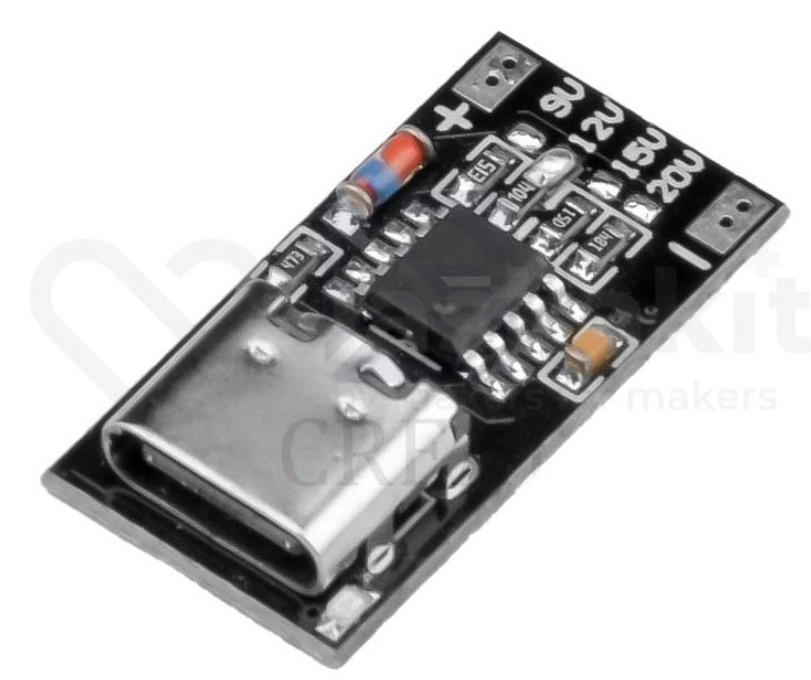
\includegraphics[width=1\textwidth]{img/PDtrig.jpg}
  \caption{\label{fig:PDtrig} Power Delivery trigger board; Převzato z~\cite{laskakit-PD}}
  \end{minipage}\hfill
  \begin{minipage}{0.3\textwidth}
    \centering
  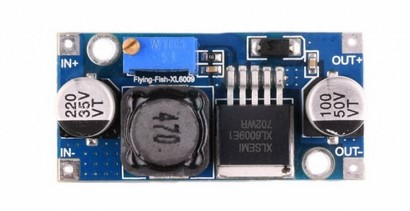
\includegraphics[width=1\textwidth]{img/XL6009.jpg}
  \caption{\label{fig:XL6009} step-up měnič s čipem XL6009; Převzato z~\cite{laskakit-XL6009}}
  \end{minipage}
  \begin{minipage}{0.3\textwidth}
    \centering
    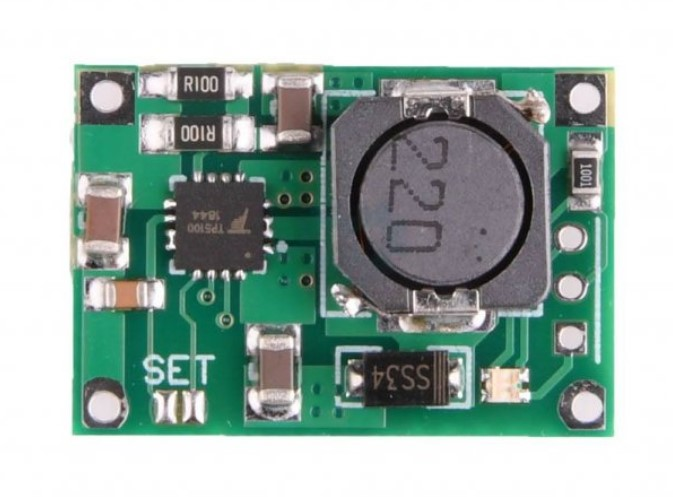
\includegraphics[width=0.8\textwidth]{img/TP5100.jpg}
    \caption{\label{fig:TP5100} Modul nabíječky dvou sériově zapojených Li-ion baterií; Převzato z~\cite{laskakit-TP5100}}
  \end{minipage}
\end{figure}

\subsubsection{Step up měnič s čipem XL6009}
Pokud ovšem připojený adaptér nepodporuje žádný rychlonabíjecí protokol, na výstupech desky bude napětí pouze 5~V Na kterém standartně běží USB připojení. Proto je k PD trigger board připojen step-up měnič nastavený na 9~V.
Pokud z PD desky bude vycházet napětí 5V, step-up jej zvýší na 9V. Pokud z PD desky bude vycházet 12V, napětí step-up projde beze změny.

\subsubsection{tp5100}
K ovládání průběhu nabíjení byl využit modul pro nabíjení Li-ionových baterií s čipem TP5100. Ten zajišťuje konstantní proud a napětí, které posílá na kontakty BMS obvodu. Další z jeho funkcí je automatické ukončení nabíjení ve chvíli, kdy baterie dosáhnou napětí 8.4~V. Je to jedinečný modul, který umožňuje nabíjení dvoučlánkových lithium-iontových akumulátorů.

\subsection{Vypínač}
K bateriím je neustále připojený jen BMS modul a nabíjecí obvod, všechny ostatní obvody jsou přemostěny vypínačem. Je tedy možné baterie nabíjet i když jsou všechny ostatní obvody odpojené. Vypínač je vidět na obrázku~\ref{fig:hw_charging_circuit}.

\subsection{Napěťové větve}
Různé komponenty projektoru pracují s různými napětími. Je tedy potřeba napětí baterií převést na několik napěťových větví. Jedná se o větve:

\begin{itemize}
  \item 5V --- Napětí Raspberry Pi, LCD a relé modulu; Zajištěno step-down měničem s čipem XL4005 (Viz obrázek~\ref{fig:XL4005}.)
  \item 12V --- Napětí Laserového modulu; Zajištěno step-up měničem s čipem MT3608 (Viz obrázek~\ref{fig:MT3608}.)
  \item symetrické napětí $\pm{}15$~V --- Napětí řídící desky galvanmetrů; Kladná větev zajištěna step-up měničem s čipem XL6009 (Viz obrázek~\ref{fig:XL6009}.), záporná větev zajištěna obvodem zdroje -15~V na HAT DPS (Viz kapitola~\ref{sec:negative-ps})
\end{itemize}


\begin{figure}[htb]
  \centering
  \begin{minipage}{0.45\textwidth}
    \centering
  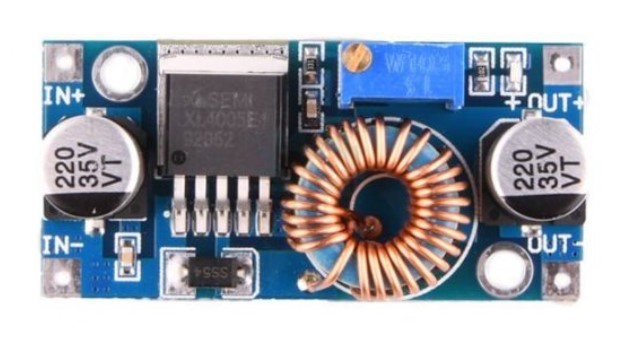
\includegraphics[width=0.8\textwidth]{img/XL4005.jpg}
  \caption{\label{fig:XL4005} step-down měnič s čipem XL4005; Převzato z~\cite{laskakit-XL4005}}
  \end{minipage}\hfill
  \begin{minipage}{0.45\textwidth}
    \centering
  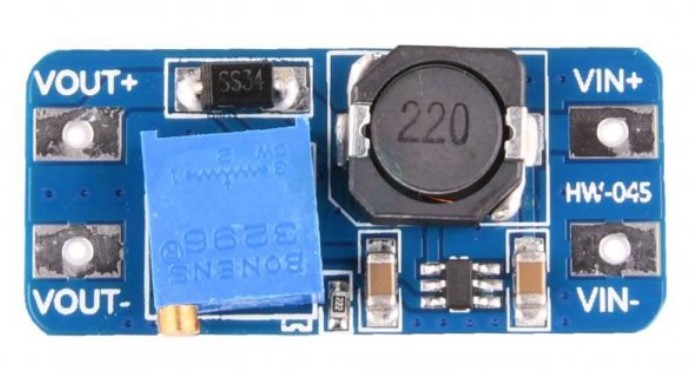
\includegraphics[width=0.8\textwidth]{img/MT3608.jpg}
  \caption{\label{fig:MT3608} step-up měnič s čipem MT3608; Převzato z~\cite{laskakit-MT3608}}
  \end{minipage}
\end{figure}


\section{Pouzdro}

V~rámci popularizace technologie se~může hodit projektor předvádět na~různých místech. Proto bude potřeba, aby~byl projektor přenosný a~při přemisťování se~nerozbil.

Pouzdro je~tedy navrženo tak, aby~bylo odolné proti nárazům a~zachovalo všechny součásti v~bezpečí. Každá součástka má své místo, kde~je~držena ze~všech stran. Pro~výrobu pouzdra by~bylo vhodné využít technologii 3D tisku. Ta~umožňuje tvorbu komplexních geometrických tvarů přímo pro~potřeby konkrétního modelu a~zároveň umožňuje snadnou iteraci a~úpravu designu pouzdra při nalezení chyb.

Pouzdro bylo navrženo v~programu Autodesk Fusion.

\subsection{Priority designu} \label{sec:krabick-design-priorities}
\subsubsection{Chlazení}
Největší část projektoru je~hliníkový chladič s~větrákem. Už od~začátku práce byl~tento chladič vybrán, aby~byl připevněn k~řídící desce galvanometrů. Problematika jejího zahřívání je~popsaná v~kapitole~\ref{sec:galvoboard-chips-heating-up}.
Jak bylo popsáno v~této kapitole, na~řídící desce galvanometrů je~připevněna hliníková destička, která chladí čipy. Chladič byl~připevněn právě na~ni.

Aktivní chladič\footnote{Chladič s~větrákem, který aktivně vytváří proud vzduchu.} se~ale~hodí i~pro~ostatní součástky. Vzduch, který nasaje, je~totiž distribuován celou vnitřní konstrukcí projektoru a~chladí tak~všechny vnitřní součástky. Tomuto proudění byla věnována zvláštní pozornost při designu konstrukce pouzdra.

\subsubsection{Přístup k~portům Raspberry Pi}
Aby bylo možné je~používat, je~potřeba zajistit jednoduchý přístup k~portům Raspberry Pi. Dále je~potřeba od~nich odlišit nabíjecí port.

\subsubsection{Modularita, jednoduchá konstrukce}
Pouzdro bylo designováno, také aby~bylo modulární. Aby~bylo možné při prototypování vyměnit pouze jednu součástku, která nesedí, místo tisknutí celého pouzdra od~začátku. S~modularitou bylo zároveň dosaženo jednoduché konstrukce, v~jakékoliv části stavby je~možné dočasně odstranit díly, aby~bylo možné upravit připevnění vnitřní elektroniky.

\subsection{Konstrukce}
Pouzdro se~skládá ze~čtyř vertikálních stěn s~otvory, do~kterých zapadají horizontální desky. Horizontální desky v~sobě mají vždy z~vrchní strany vyhloubené prohlubně, do~kterých pasují elektronické součástky, které na~nich leží. Díky tomu se~elektronické součástky při pohybu projektoru volně nepohybují ve~vnitřních prostorách.

\begin{figure}[htb]
  \centering
  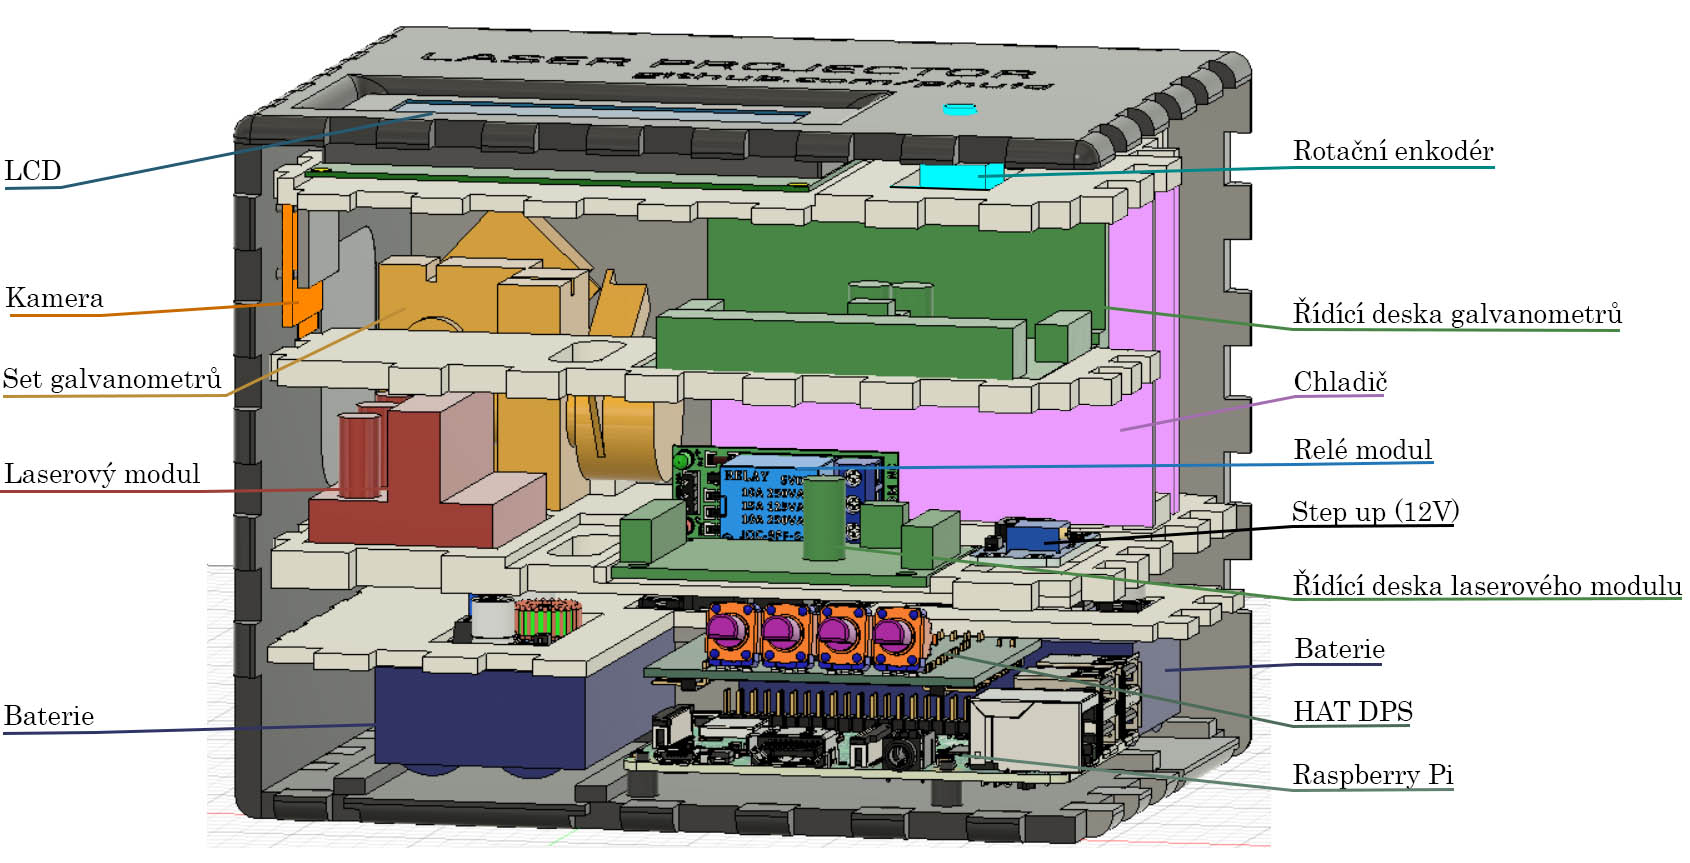
\includegraphics[width=1\textwidth]{img/case-sideview.jpg}
  \caption{\label{fig:case-sideview} Pohled do~projektoru s~odstraněnou přední stěnou v~programu Autodesk Fusion}
\end{figure}

Tyto prohlubně jsou hlavní důvod, proč byl~k~výrobě dílů využit 3D tisk místo například laserového řezání.

Elektronika je~v~prohlubních často držena i~lepidlem z~tavné pistole.
To bylo přidáno s~původním cílem upevnit k~elektronice kabely z~ní vedoucí i~za~izolaci. Kdyby kabely držely jen~za~vodičové drátky k~elektronice připájené, drátky by~se~v~průběhu času kvůli vibracím při přenášení polámaly.

Jak je~vidět na~obrázku~\ref{fig:case-sideview}, pouzdro je~rozděleno do~pěti pater. Jednotlivá patra nezabírají celou horizontální plochu projektoru. Často spojují pouze tři ze~čtyř stěn, nebo jsou v~nich otvory, kterými může proudit vzduch. V~prvním patře se~nachází baterie (zvýrazněny modře), destička s~BMS obvodem a~v~neposlední řadě Raspberry Pi.
Na~něm je~připevněná HAT~deska plošných spojů, která zasahuje do~druhého patra. Druhé patro je~vidět na~obrázku~\ref{fig:hw_layer0} a~nachází se~v~něm obvod nabíjení baterie (PD trigger deska, step up~měnič a~nabíječka Li-ion článků).
Dále se~v~něm nachází step down měnič napájející Raspberry Pi~a~step up~měnič napájející galvanometry.
\fxnote{tecka @ obr.\ref{fig:hw_layer0}} 
\begin{figure}[htb]
  \centering
  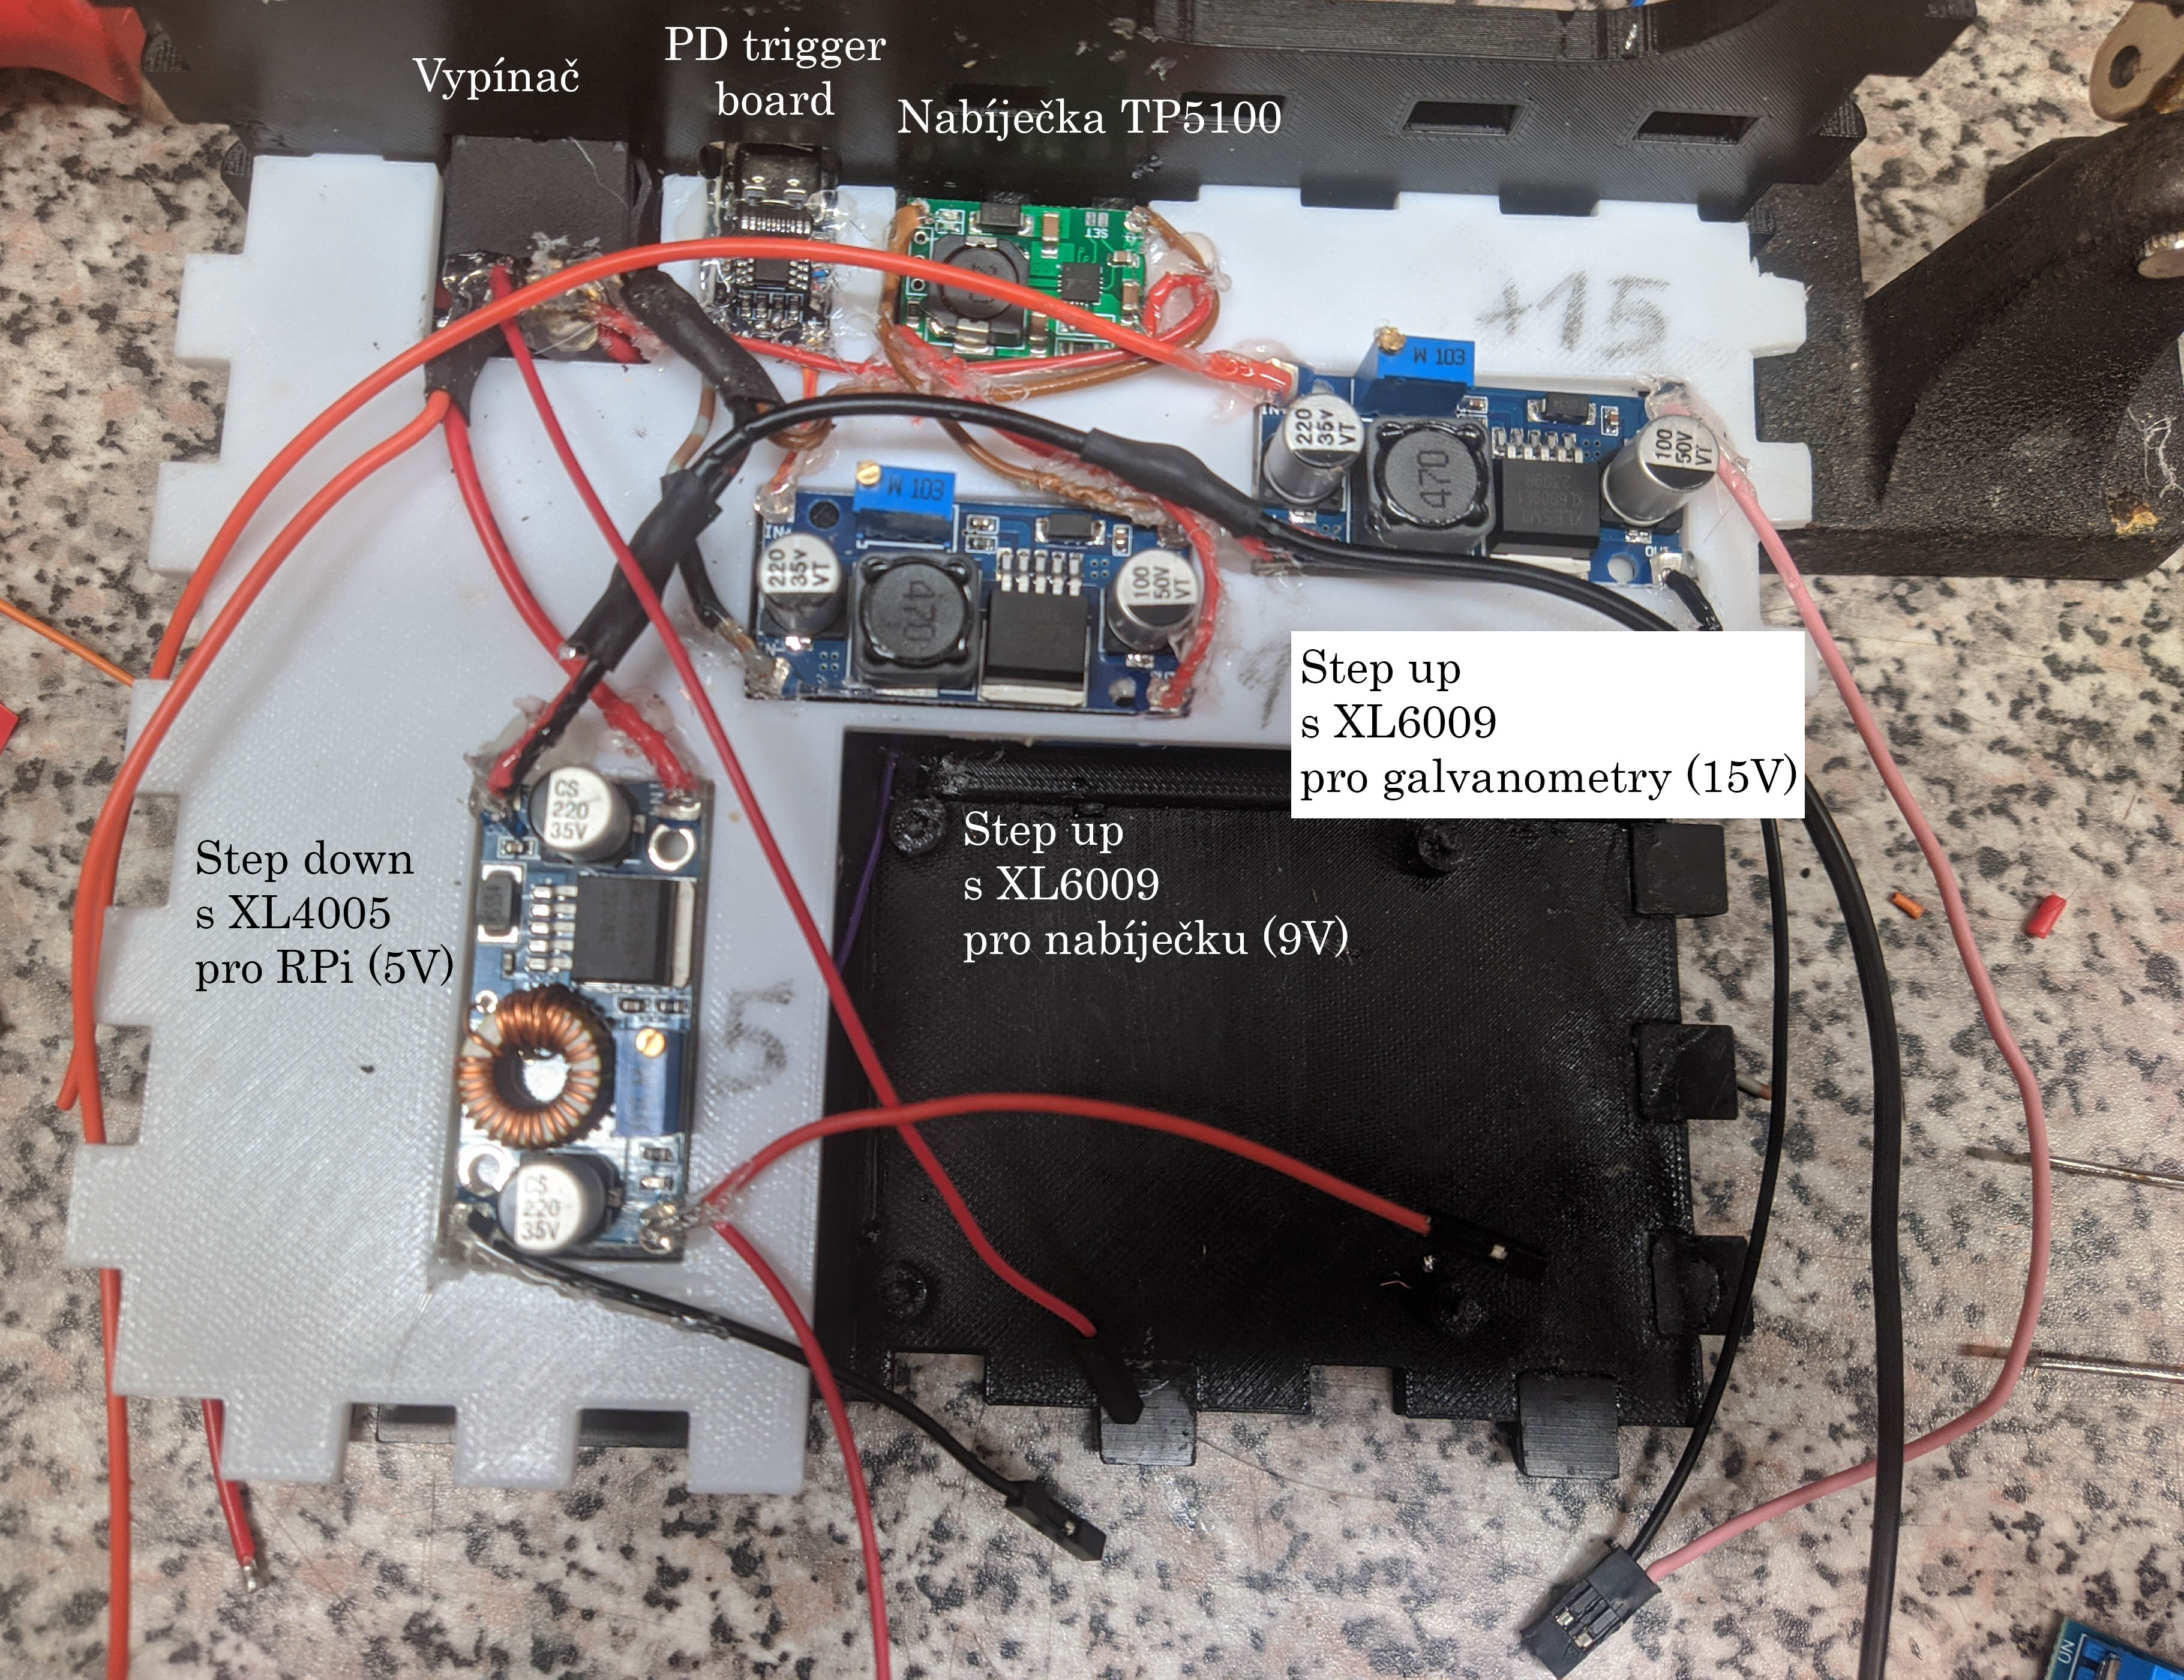
\includegraphics[width=0.8\textwidth]{img/hw_layer0.jpg}
  \caption{\label{fig:hw_layer0} Kompletně nainstalované druhé patro (Na obrázku je~modul TP5100 zapojen s~opačnou polaritou, ve~výrobku byla chyba opravena, ale~tato fotka je~stále nejlepší ilustrace.)}
\end{figure}

Ve třetím patře je~upeněn chladič, foukající na~nabíjecí obvod a~step up~měniče pod~ním, set~galvanometrů (zvýrazněn žlutě), laserový modul (zvýrazněn červeně) a~jeho řídící deska (zvýrazněna zeleně), step up~měnič pro~laser a~relé modul.  
Galvanometry zasahují až do~čtvrtého patra, kde~je~upevněna jejich řídící deska. Ta~je~mimo jiné připevněna na~chladič párem šroubků viditelných na~obrázku~\ref{fig:hw_galvoboard} ze~strany \pageref{fig:hw_galvoboard}, mezi desku a~chladič byla aplikována teplovodivá pasta. V~prostorách čtvrtého patra je~také na~stěnu upevněna kamera.
V pátém patře se~nachází LCD~a~rotační enkodér.

V horizontálních deskách oddělujících patra od~sebe jsou otvory pro~vzduch, jak~je~zmíněno v~sekci~\ref{sec:krabick-design-priorities}, také na~přední stěně pouzdra jsou otvory pro~vyfukování vzduchu. Na~přední stěně je~také otvor pro~přístup k~potenciometrům na~HAT~DPS a~otvor pro~přístup k~portům Raspberry Pi, ten~je~i~na~pravé boční stěně.
Na~zadní stěně je~otvor pro~nasávání vzduchu větrákem, vypínač a~otvory pro~USB-C port PD~trigger desky a~statusové diody nabíječky TP5100. Na~levé boční stěně jsou pak~otvory pro~kameru a~laserový výstup galvanometrů. Ve~dně jsou otvory pro~výmněnu baterií a~ve~stropní stěně jsou otvory pro~LCD a~rotační enkodér.

\begin{figure}[htb]
  \centering
  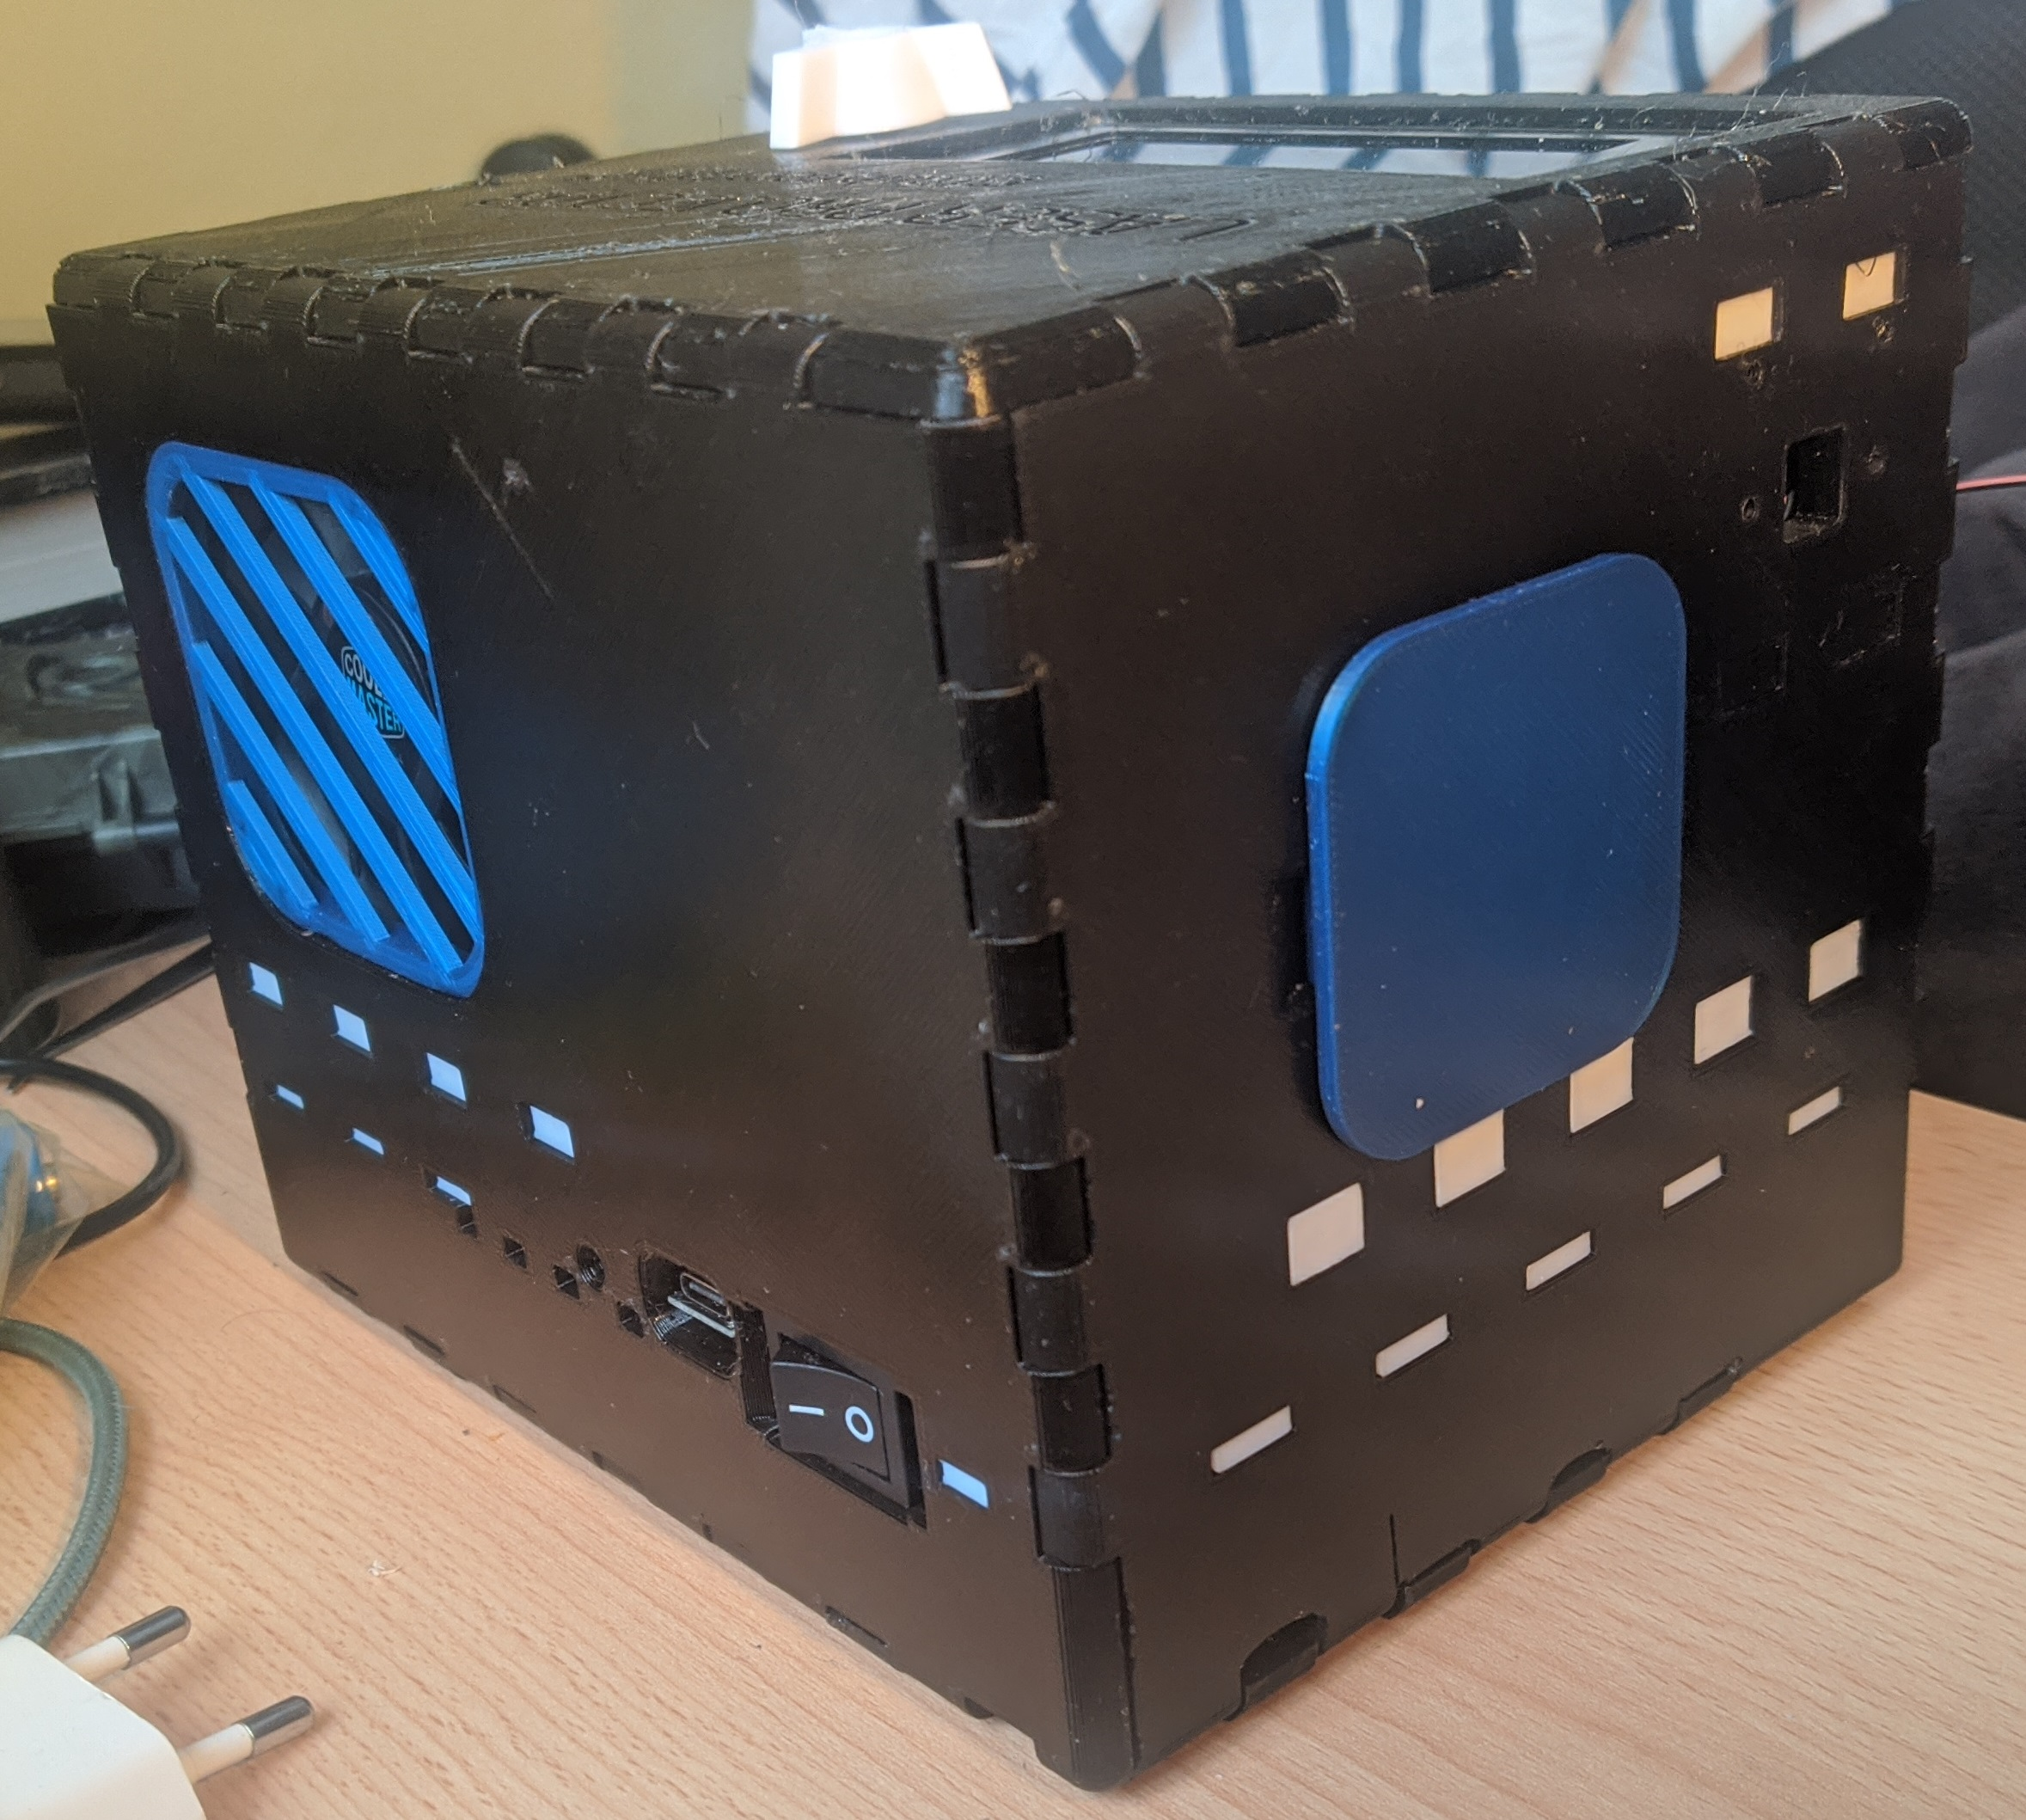
\includegraphics[width=0.8\textwidth]{img/hw_sides_backleft.jpg}
  \caption{\label{fig:hw_sides_backleft.jpg} Pohled na~projektor ze~strany hrany sousedící se~zadní a~pravou boční stěnou}
\end{figure}

\fxnote{fotka zepredu a~zprava}



\fxnote{TODO cos udelal svyho vlastne a~jak to~facha}

\section{cooler}

\section{napájení}
\fxnote{TODO ay~tak co, zvladls to~dat na~baterky?}


% !TeX root = text.tex
\chapter{Software}

Tato kapitola se~zabývá softwarovou výbavou laserového projektoru. Popisuje klíčové programy, jejich funkce a~způsob, jakým mezi sebou komunikují.
Mezi tyto programy patří program lasershow, který obsluhuje vykreslování, programy pro~interakci s~uživatelem (dále \uv{frontendové programy}) jako UI, web\_ui a~discord\_bot, a~také program wifi\_manager, který spravuje wifi připojení Raspberry Pi.
Programy wifi\_manager a~lasershow se~dají označit za~backendové programy, protože neinteragují s~uživatelem.

V neposlední řadě popisuje také instalační skript, který výrazně zjednodušuje instalaci všech zmíněných programů a~jejich závislostí.

Program lasershow umí číst projekční soubory ve~formátu .ild.
Uživatel může takový soubor vytvořit například v~softwaru Laserworld Showeditor V7~\cite{showeditor} nebo může do~frontendových programů nahrát soubor v~populárním vektorovém formátu .svg a~frontendové programy využijí skript svg2ild.py dostupný~z~\cite{svg2ild}.

% O~řízení galvanometrů se~stará program lasershow, který je~psaný v~jazyce c++ pro~maximální rychlost. Tento program běží na~pozadí a~čeká na~příkazy od~programů určených k~interakci s~uživatelem. Na~tento program se~zaměřuje kapitola lasershow. \fxnote{TODO: odkaz}

% Dále jsou tu~programy, které se~starají o~interakci s~uživatelem. Tyto programy přijímají příkazy od~uživatele a~posílají je~programu lasershow. Navíc od~lasershow získávají výstup, který následně zprostředkovávají uživateli; důkladněji popsáno v~kapitole~\ref{sec:comms}.
% Mezi tyto programy patří programy UI, web\_ui a~discord\_bot. Program UI~spravuje OLED displej, přijímá od~uživatele vstup rotačním enkodérem a~je~psaný v~c++ pro~jednodušší interakci s~hardwarem. Program web\_ui využívá runtime Node.js, ve~kterém je~nenáročné vytvořit http server dostupný z~lokální sítě. \fxnote{(A)?} Program discord\_bot, také využívající Node.js, přijímá příkazy z~chatovací aplikace discord a~je~přístupný i~přes internet.

% Nakonec je~tu~program wifi\_manager, ten~spravuje wifi připojení RPi, je~psaný v~Node.js a~komunikuje s~programy, které interagují s~uživatelem stejně jako program lasershow.

\section{komunikace mezi programy}\label{sec:comms}
Všechny tyto programy jsou propojeny síťovými sockety zprostředkovanými knihovnou ZeroMQ, která nabízí frontu\footnote{Ve frontě jsou zprávy seřazeny od~té nejdříve odeslané.} zpráv, bez potřeby samostatně běžícího brokeru.

Tato knihovna je~využita k~vytvoření dvou socketů, jedním lasershow přijímá příkazy od~uživatele prostřednictvím ostatních programů (vstupní socket na~portu 5557, viz obr.~\ref{fig:tcp5557}) a~do~druhého posílá informace ostatním programům (výstupní socket na~portu 5556, viz obr.~\ref{fig:tcp5556}), aby je~zprostředkovaly uživateli.
Do~prvního zmíněného posílají progamy interagující s~uživatelem příkazy pro programy lasershow a~wifi\_manager. Do~druhého posílá lasershow informace o~stavu a~změnách nastavení  a~také wifi\_manager informace o~stavu a~změnách v~nastavení WiFi.

Příkazy pro programy lasershow a~wifi\_manager vypadají následovně
\fxnote{TODO: příklady příkazů pro lasershow a~wifi\_manager z~\url{https://github.com/phuid/laser_projector/blob/master/README.md}}
\fxnote{TODO: příklady status infos od~lasershow a~wifi\_manager z~\url{https://github.com/phuid/laser_projector/blob/master/README.md}}

\begin{figure}[htb]
  \centering
  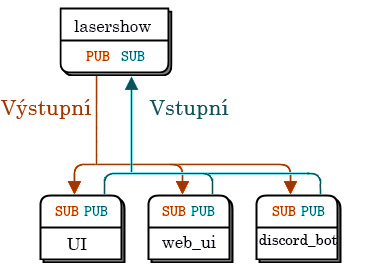
\includegraphics[width=0.5\textwidth]{img/comms_lasershow_scheme.jpg}
  \caption{\label{fig:lasershow_comms} Komunikace mezi programy vstupním socketem na~portu 5557}
\end{figure}
\begin{figure}[htb]
  \centering
  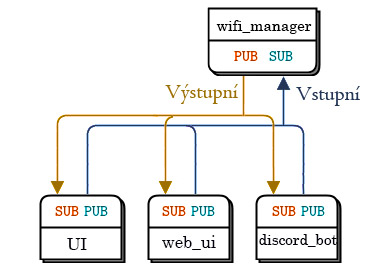
\includegraphics[width=0.5\textwidth]{img/comms_wifiman_scheme.jpg}
  \caption{\label{fig:wifiman_comms} Komunikace mezi programy výstupním socketem na~portu 5556}
\end{figure}

\section{lasershow}

Program lasershow je~psaný v~jazyce c++, který je~kompilovaný a~obecně považovaný za~jeden z~nejrychlejších jazyků. Druhé zmíněné se~hodí, jelikož chceme vykreslovat co~možná nejrychleji.

Tento program zaregistruje vstupní TCP socket na~portu 5557 a~knihovnou ZeroMQ se~na něm přihlásí k~odběru zpráv, které do~něj publikují ostatní programy. Zárověn podobně zaregistruje výstupní socket na~portu 5556, do~kterého později bude posílat zprávy pro programy, které interagují s~uživatelem.

Následně se~připojí k~DAC a~čeká na~zprávy od~ostatních programů. Jakmile zprávu obdrží, zpracuje ji~a pokud je~požadována změna nastavení, okamžitě ji~provede a~aktuální nastavení si~uloží do~souboru, jestliže je~požadováno vykreslení obrazu ze~souboru, začne obraz vykreslovat. Při tom průběžně posílá informace o~stavu vykreslování do~výstupního socketu. I~při vykreslování obrazu tento program zpracovává zprávy a~pokyny ze~vstupního socketu.

Program byl původně převzat z~projektu \url{https://github.com/tteskac/rpi-lasershow}\footnote{staženo 28.~12.~2023}, následně byl ale přepsán skoro ve~všech ohledech a~z původního programu zbylo asi 20 řádků.
\fxnote{TODO: odkud jsem to~vzal a~prepsal a~jak moc jsem toho udelal a~s jakymy vysledky}

\fxnote{TODO: diagram programu}

\fxnote{TODO: priklad zmq}\

\fxnote{ use \url{https://cs.overleaf.com/learn/latex/Code_Highlighting_with_minted} instead - function highlights}

\lstinputlisting[language=c++, style=code]{code_examples/zmq_server.cpp}
\lstinputlisting[language=c++, style=code]{code_examples/zmq_client.cpp}


\section{wifi\_manager}

V rámci této práce byl vyvinut ještě jeden program, který se~přímo nepodílí ani na~projekci, ani na~interakci s~uživatelem.

Program wifi\_manager je~také napsaný v~jazyce JavaScript s~využitím runtime Node.js. Registruje se~ke stejným socketům jako lasershow, přijímá příkazy týkající se~nastavení WiFi na~Raspberry Pi~TCP socketem na~portu 5557 a~odesílá zpětnou vazbu na~TCP socket s~portem 5556.

\fxnote{TODO: jak se~komunikace s~lasershow odlisuje od~wifi\_managera}

\fxnote{TODO: ukazka(idk what)}

Hlavním úkolem tohoto programu je~správa a~konfigurace WiFi připojení na~Raspberry Pi. Přijímá příkazy od~ostatních programů a~nastavuje WiFi parametry na~základě těchto příkazů. Tím umožňuje uživatelům snadno a~pohodlně nastavit WiFi připojení na~svém zařízení.

Stejně jako lasershow, wifi\_manager také posílá zpětnou vazbu ostatním programům, aby informoval o~stavu a~změnách v~nastavení WiFi. Tímto způsobem je~zajištěna komunikace a~synchronizace mezi všemi programy v~laserovém projektoru.

Celkově wifi\_manager přispívá k~plynulému a~efektivnímu provozu laserového projektoru tím, že umožňuje snadnou správu a~konfiguraci WiFi připojení na~Raspberry Pi.

\section{UI}
Program UI~je~také psaný v~jazyce c++ a~. Tento program ovládá OLED displej, který je~připojený na~Raspberry Pi~pomocí rozhraní I2C, a~přijímá vstup od~uživatele čtením rotačního enkodéru s~tlačítkem. Také příjmá informace od programů lasershow a wifi\_manager a posílá jim vstup od uživatele.

Na LCD displeji má uživate ldíky tomuto programu přístup k menu, kde jsou zobrazeny aktuální informace o promítání a wifi připojení a kde uživatel může měnit nastavení dvou backendových programů.

\subsection{Využité knihovny}
\subsubsection{wPi\_soft\_lcd}
Hlavní využitou knihovnou je wPi\_soft\_lcd~\cite{wpi-lcd}. Tato knihovna umožňuje jednoduchou komunikaci s LCD prostřednictvím I$^{2}$C převodníku. 

Mezi nejdůležitější funkce této knihovny, které používám ve svém kódu patří:
\begin{itemize}
  \item \mintinline{cpp}{lcd_t *lcd_create(int scl, int sda, int addr, int lines)} --- Tato funkce inicializuje komunikaci s I$^{2}$C převodníkem. Je nutné ji zavolat před jiným použitím knihovny. Příjmá čísla pinů I$^{2}$C sběrnice, na které je připojený displej, dále příjmá I$^{2}$C adresu převodníku a počet řádků displeje. Funkce vrací pointer na nově vytvořenou strukturu typu \mintinline{cpp}{lcd_t}, který je potřeba k volání dalších funkcí knihovny. Jestliže se nepodaří inicializovat knihovnu, vrací hodnotu \mintinline{cpp}{NULL}.
  \item \mintinline{cpp}{void lcd_printf(lcd_t *lcd, const char* format, ... )} --- K vypsání textu na LCD využívám tuto funkci. Příjmá pointer vrácený funkcí \mintinline{cpp}{lcd_create}, formátovací řetězec a případně další argumenty stejně, jako známá funkce \mintinline{cpp}{printf} ze standartní knihovny programovacího jazyka C.
  \item \mintinline{cpp}{void lcd_clear (lcd_t *lcd)} --- Funkce při jejím zavolání vymaže všechen text zobrazený na LCD. Příjmá pointer funkcí \mintinline{cpp}{lcd_create}.
  \item \mintinline{cpp}{void lcd_pos(lcd_t *lcd, int row, int col)} --- Touto funkcí je možno nastavit pozici virtuálního kurzoru, od kterého začne vypisovat funkce \mintinline{cpp}{lcd_printf}. Příjmá  pointer funkcí \mintinline{cpp}{lcd_create}, číslo řádku a číslo sloupce požadované pozice kurzoru. Obě čísla jsou počítaná od nuly.
  \item \mintinline{cpp}{void lcd_backlight_dim (lcd_t *lcd, float intensity)} --- Funkce, která nastaví střídu PWM signálu na GPIO pinu 18 a tím reguluje jas podsvícení LCD. Příjmá pointed vrácený funkcí \mintinline{cpp}{lcd_create} a desetinné číslo od 0 do 1, značící požadovanou intenzitu podsvícení.
  \item \mintinline{cpp}{void lcd_create_char(lcd_t *lcd, int n, char *data)} --- Touto funkcí je možné definovat vlastní znaky, které se zobrazí na LCD. Příjmá pointer vrácený funkcí \mintinline{cpp}{lcd_create}, číslo znaku, který má být definován a pole 8 bytů, které reprezentuje vlastní znak.
  \item \mintinline{cpp}{}
  \item \mintinline{cpp}{}
  \item \mintinline{cpp}{}
  \item \mintinline{cpp}{}
\end{itemize}

\subsubsection{wiringPi}
Předchozí popsaná knihovna pro posílání signálu I$^{2}$C sběrnicí používá knihovnu wiringPi, která umožňuje ovládání GPIO pinů. Abych nepřidával do jednoho programu dvě knihovny interagující s hardwarem, stejnou knihovnu využívám pro čtení dat z enkodéru.

Je nepraktické využívat v tomto programu jinou knihovnu na interakci s hardwarem, proto v budoucnu přepíši knihovnu wPi\_soft\_lcd tak, aby i ona využívala modernější knihovnu pigpio popsanou v kapitole \ref{sec:ls_pigpio}.

\begin{itemize}
\item \mintinline{cpp}{void pinMode (int pin, int mode)} --- Funkce, která pro GPIO pin z argumentu \mintinline{cpp}{pin} nastaví mód z argumentu \mintinline{cpp}{mode}. Jako argument \mintinline{cpp}{mode} používám hodnotu \mintinline{cpp}{INPUT}, která pin zaregistruje pro vstup.
\item \mintinline{cpp}{void pullUpDnControl (int pin, int pud)} Funkce připojí na pin \mintinline{cpp}{pin} pull-up nebo pull-down rezistor podle argumentu \mintinline{cpp}{pud}. Jako argument \mintinline{cpp}{pud} používám hodnotu \mintinline{cpp}{PUD_UP}, která k pinu připojí pull-up rezistor.
\item \mintinline{cpp}{int wiringPiISR (int pin, int mode, void (*function)(void))} --- Tato funkce nastaví přerušení na pin \mintinline{cpp}{pin}. Tak, aby při změně hodnoty na tomto pinu byla zavolána tzv. callback funkce z argumentu \mintinline{cpp}{function}. Argument \mintinline{cpp}{mode} úrčuje, jestli je funkce zavolána pouze při tzv. rising edge, tzv. falling edge, nebo při obou. Já v tomto argumentu používám hodnotu \mintinline{cpp}{INT_EDGE_BOTH}.
\end{itemize}

\subsubsection{cppzmq}
Samozřejmě program také využívá knihovnu cppzmq dostupnou z \cite{cppzmq} a popsanou v kapitole \ref{sec:ls_cppzmq}. Program ji používá podobně jako program lasershow, ne však stejně.

Největším rozdílem je, že místo funkce \mintinline{cpp}{void zmq::socket_t::bind} používá funkci \mintinline{cpp}{void zmq::socket_t::connect(const char *addr_)}.
Funkci bind je totiž potřeba zavolat přesně jednou pro každý socket.
Jestliže ji už pro sockety zavolal program lasershow a socket tedy už je registrovaný k danému portu, je třeba zavolat funkci \mintinline{cpp}{connect}.

Dále samozřejmě stejně jako všechny frontendové programy do vstupního socketu zprávy posílá a z výstupního socketu zprávy čte.

\subsection{Struktura programu}
Program začne inicializací komunikace s LCD.
Poté pokračuje registrací interruptů na pinech, ke kterým je připojen enkodér. A následně se připojí k socketům aplikací lasershow a wifi\_manager.

V další části programu je definováno samotné menu. To má podobu struktury \mintinline{cpp}{menu_option}, která je definována následovně.

\begin{minted}{cpp}
struct menu_option
{
  std::string name;

  std::string command_name;

  menu_option_style style = UNDEFINED;

  std::vector<menu_option> nested_menu_options = {};
  uint8_t nest_selected = 0;
  uint8_t nest_scroll = 0;
  bool nest_option_active = 0;
  bool redraw = 0;

  menu_val<float> value;

  bool has_function = 0;
  void (*function)(zmq::socket_t &, menu_option &);
};
\end{minted}

Díky ní může definice menu vypadat například takto:

\begin{minted}{cpp}
  menu_option root = {
        .name = "ROOT",
        .style = ROOT_MENU,
        .nested_menu_options = {
            {
                .name = "progress%",
                .command_name = "progress",
                .style = VALUE,
                .value = {0, 0, 100, 0.5},
            },
            {
                .name = "current_frame",
                .command_name = "current_frame",
                .style = VALUE,
                .value = {1, 1, 1, 1},
            },
            {.name = "-no out received-",
             .style = TEXT},
            {.name = "STOP",
             .command_name = "STOP",
             .style = TEXT,
             .has_function = 1,
             .function = send_option_command},
            {.name = "PAUSE", .command_name = "PAUSE", .style = TEXT, .has_function = 1, .function = send_option_command},
            {
                .name = "PROJECT",
                .style = NESTED_MENU,
                .has_function = 1,
                .function = fill_with_files,
            },
            {
                .name = "options",
                .style = NESTED_MENU,
                .nested_menu_options = {
                    {
                        .name = "screen brightness",
                        .command_name = "screen_brightness",
                        .style = VALUE,
                        .value = {50, 0, 100},
                    },
                    {
                        .name = "repeat",
                        .command_name = "repeat",
                        .style = VALUE,
                        .value = {0, 0, 1, 1},
                    },
                    {
                        .name = "point_delay",
                        .command_name = "point_delay",
                        .style = VALUE,
                        .value = {0, 0, 10000, 10},
                    },
                    {
                        .name = "target_frame_time",
                        .command_name = "target_frame_time",
                        .style = VALUE,
                        .value = {0, 0, 10000, 1},
                    },
                    {
                        .name = "trapezoid_horizontal",
                        .command_name = "trapezoid_horizontal",
                        .style = VALUE,
                        .value = {0, -1.f, 1.f, 0.05},
                    },
                    {
                        .name = "trapezoid_vertical",
                        .command_name = "trapezoid_vertical",
                        .style = VALUE,
                        .value = {0, -1.f, 1.f, 0.05},
                    },
                },
                .has_function = 1,
                .function = read_options,
            }}};
\end{minted}

Následuje nekonečný cyklus, ve kterém program příjmá zprávy od programů lasershow a wifi\_manager a volá funkci menu\_interact, kter

\subsection{vysledekdsdsa}

\section{web\_ui}

Narozdíl od~předchozích dvou zmiňovaných programů je~program web\_ui psaný v~jazyce javascript, ten nepatří mezi nejrychlejší, ale díky runtime Node.js a~knihovnám http a~formidable v~něm bylo časově nenáročné vytořit http web server.

Tento server běží na~portu 3000 a~je~dostupný z~lokální sítě (tzn. přímo z\~Raspberry Pi~na~adrese http://localhost:3000 nebo z~jakéhokoliv zařízení na~stejné lokální síti na~ip~adrese RPi).
Program je~využíván pro jednoduchou interakci s~uživatelem, který může pomocí webového prohlížeče ovládat laserový projektor pár kliknutími i~zadávat vlastní příkazy klávesnicí.

\fxnote{na webu jsou konzole pro ssh, wifiman a~lasershow, taky fast project forms, queue, settings, a chtel jsem pridat i kamerove online ukozovatko}

\fxnote{TODO: příklad http serveru}
\inputminted{js}{code_examples/http_static_files.js}

Stejně jako program UI~za~pomoci knihovny ZeroMQ tento program odebírá z~výstupního socketu zprávy o~průběhu vykreslování od~programu lasershow a~odesílá mu~pokyny uživatele na~vstupní socket.

\fxnote{TODO: příklad přihlášení k~socketům v~js}

\fxnote{TODO: xterm + ssh}

\section{discord bot}

Posledním programem, který je~využíván k~interakci s~uživatelem je~discord\_bot, který je~také psaný v~jazyce javascript v~runtime Node.js, stejně jako předchozí programy se~přihlásí k~socketům knihovnou zmq, ale na~rozdíl od~nich tento program může interagovat s~uživatelem přes internet ať už je~kdekoliv na~světě.
Pomocí knihovny discord.js se~přihlásí k~předem vytvořenému bot účtu, který může na~předem vytvořeném discord serveru čekat na~zprávy od~uživatele, ty~posílat do~vstupního socketu a~posílat uživateli zpětnou vazbu, kterou příjme z~výstupního socketu.



\section{Instalační skript}
Nedílnou součástí softwarové výbavy projektoru je~instalační skript.
Ten je~psaný v~příkazovém jazyce bash, který odpovídá sekvenci příkazů v~příkazovém řádku.
Instalační skript umožňuje instalaci celého projektu pouze třemi příkazy, viz~ukázka kódu~\ref{list:install-commands}.

\begin{code}
  \captionof{listing}{\label{list:install-commands} Příkazy potřebné k~instalaci projektu}
\begin{minted}[frame=lines,fontsize=\footnotesize,linenos]{shell}
   git~clone https://github.com/phuid/laser_projector.git
  cd~laser_projector
  bash install.sh
\end{minted}
\end{code}

Instalační skript stáhne a~nainstaluje nainstaluje veškeré závislosti a~knihovny ostatních programů. Stáhne také samotný interpreter Node.js.
Následně zkompiluje programy psané v~c++ a~nainstaluje a~nastaví služby potřebné k~vysílání hotspotu. Poté pomocí manažeru procesů pm2 dostupného z~\cite{pm2} nastaví automatické zapínání ostatních programů a~po~potvrzení uživatelem systém restartuje, aby~provedené změny nabyly efekt.


\fxnote{TODO udelals to vubec dobre? porovnej se s ostatnima}
\chapter{Diskuze}
\section{ruzne technologie}
\cite{scanning-handbook} str. 394 \\
Digital micromirror devices (DMDs) and
liquid crystal displays (LCDs) have also captured the field of image projection away from
oscillating scanners.
uz existuje MEMS - pcb, co ma X i Y v jednom zrcatku, je super a vsechno jiny prave nahrazuje, na user levelu je i docela podobny galvum - jedna civka x druha y - overit,, idk, jesti tam civky nejsou proste pod tim a nejenom v kloubech


\fxnote{kam pokracovat: api p
ro random programy - aby si mohli pokrocilejsi kutilove taky hrat a randomly posouvat laser ig}

\section{další zpracování tématu}
udelal jsem to dobre? vybral jsem si dobry technky?
like byl by lepsi ten harddrive z yt?
nebo fakt to melo byt napajeny z baterek a ne ze zasuvky?

ze hej ze \href{https://dspace.vutbr.cz/bitstream/handle/11012/38621/final-thesis.pdf?sequence=-1}{typek z vut} udelal kinda kurva podobnej HW jak ja, ale ja to mam trochu jinak, cuz jsem o tom nevedel, ale ofc moje je lepsi :))
also to delala hromada dalsich lidi na internetu ten hw, also od gh.com/tteskac mam executable, kterou jsem ale totalne ze rozsiril a taky jsem pridal vsechno moje genialni ui muhahahah

\B{ze este dalsi zpracovani: (19.10.2023 vsechny dostupne)}
\begin{enumerate}
  \item used/modified code
        \begin{itemize}
          \item \url{https://github.com/marcan/openlase/blob/master/tools/svg2ild.py}
          \item \url{https://github.com/tteskac/rpi-lasershow}
          \item \url{https://github.com/sabhiram/raspberry-wifi-conf/blob/master/app/wifi\_manager.js}
          \item \url{http://www.electronicayciencia.com/wPi_soft_lcd/}
          \item \href{https://dspace.vutbr.cz/bitstream/handle/11012/38621/final-thesis.pdf?sequence=-1}{typek z vut}
        \end{itemize}
  \item dalsi zpracovani stejny projekty
        \begin{itemize}
          \item \url{https://www.instructables.com/Arduino-Laser-Show-With-Real-Galvos/}
          \item \url{https://github.com/tteskac/rpi-lasershow}
          \item \url{https://www.instructables.com/DIY-STEPDIR-LASER-GALVO-CONTROLLER/}
          \item \href{https://youtu.be/u9TpJ-_hBR8?si=mHy-UrptZZJ0Xu5-}{borec na yt hard-drive text gut}
        \end{itemize}
  \item other useful thingies
        \begin{itemize}
          \item \url{https://hackaday.io/project/172284-galvo-laser-cutterengraver}

          \item \url{https://hackaday.io/project/172284/instructions}

          \item \url{https://learn.adafruit.com/mcp4725-12-bit-dac-with-raspberry-pi/hooking-it-up}
          \item \url{https://www.ilda.com/resources/StandardsDocs/ILDA_IDTF14_rev011.pdf}
          \item cool demos \url{https://marcan.st/projects/openlase/}
          \item \url{https://www.youtube.com/watch?v=u9TpJ-_hBR8}
        \end{itemize}
  \item read
        \begin{itemize}
          \item \url{https://www.laserworld.com/en/glossary-definitions/90-t/2797-ttl-modulation-en.html}
        \end{itemize}

\end{enumerate}


\newpage
\chapter*{Závěr}
\addcontentsline{toc}{chapter}{Závěr} \fxnote{FIXME proc vsichni maji zaver v~obsahu jako section, kdyz pak vypada, ze~je pod posledni kapitolou??}
\fxnote{TODO závěr}\fxnote{TODO muj projekt je~dostupný na~githubu}
\fxnote{vytvoril jsem projektor, ten je~mozne sestavit s~minimální znalostí elektroniky, staci umet pajet, jde mi~o to~zajemcum predstavit jak to~programovat, jak funguji vektorove formaty, ne~jak funguje hw, ten se~totiz meni - MEMS}
\fxnote{tim ze~mam linux lasershow obcas zpomali, obcas zrychli, samozrejme mam osetreny, aby nezrychlily framy, ale pointy ano}

\newpage
\printbibliography[title=Literatura]
\addcontentsline{toc}{section}{Literatura}

\listoffigures
\addcontentsline{toc}{section}{Seznam obrázků}

\listoftables
\addcontentsline{toc}{section}{Seznam tabulek}
%
% \listoflistedequation
% \addcontentsline{toc}{section}{Seznam rovnic}

\end{document}
